% Copyright (c) 2023-2026 Oriol Cayon, Delft University of Technology
% SPDX-License-Identifier: Apache-2.0
%
% Tables, macros and all drivetrain_* figures come from
%   python scripts/identification/estimate_drivetrain_losses.py
% (generated/, figures/drivetrain_*.png). ground_station_layout.png is a
% drawing of GS1. Hardware in this note is GS1 only.
% Rebuild:  latexmk -pdf drivetrain_physics.tex   (in docs/winch/)
\documentclass[11pt,a4paper]{article}

\usepackage[margin=2.4cm]{geometry}
\usepackage{graphicx}
\usepackage{amsmath,amssymb}
\usepackage{booktabs}
\usepackage{xcolor}
\usepackage{caption}
\usepackage{float}
\usepackage{enumitem}
\usepackage{fancyhdr}
\usepackage{xurl}
\usepackage[hidelinks]{hyperref}
\usepackage{siunitx}
\usepackage{tabularx}
\sisetup{range-phrase={--},range-units=single,per-mode=power}

\graphicspath{{figures/}}
\newcommand{\cyclePtether}{6.72}
\newcommand{\cycleLossLow}{12.1}
\newcommand{\cycleLossHigh}{20.4}
\newcommand{\cycleDownLow}{11.1}
\newcommand{\cycleDownHigh}{16.7}
\newcommand{\cycleLossKWLow}{0.81}
\newcommand{\cycleLossKWHigh}{1.37}
\newcommand{\cycleNoLoadLow}{7.6}
\newcommand{\cycleNoLoadHigh}{7.6}
\newcommand{\cycleNoLoadShareLow}{37}
\newcommand{\cycleNoLoadShareHigh}{63}
\newcommand{\cycleMeshLow}{1.6}
\newcommand{\cycleMeshHigh}{3.2}
\newcommand{\cycleBeltLow}{1.6}
\newcommand{\cycleBeltHigh}{4.9}
\newcommand{\cyclePulleyLow}{1.2}
\newcommand{\cyclePulleyHigh}{4.4}
\newcommand{\peakLow}{1.6}
\newcommand{\peakHigh}{2.1}
\newcommand{\reelinShareLow}{34}
\newcommand{\reelinShareHigh}{44}
\newcommand{\allReelinShareLow}{33}
\newcommand{\allReelinShareHigh}{44}
\newcommand{\allLossKWLow}{0.59}
\newcommand{\allLossKWHigh}{1.37}
\newcommand{\allPctLow}{12.1}
\newcommand{\allPctHigh}{22.7}
\newcommand{\shaftShareLow}{77}
\newcommand{\shaftShareHigh}{88}
\newcommand{\roLossLow}{0.67}
\newcommand{\roLossHigh}{1.33}
\newcommand{\roPctLow}{5.2}
\newcommand{\roPctHigh}{10.3}
\newcommand{\roMeshLow}{74}
\newcommand{\roMeshHigh}{148}
\newcommand{\roBeltLow}{74}
\newcommand{\roBeltHigh}{222}
\newcommand{\roPulleyLow}{54}
\newcommand{\roPulleyHigh}{202}
\newcommand{\riLossLow}{0.90}
\newcommand{\riLossHigh}{1.08}
\newcommand{\rfLossLow}{3.16}
\newcommand{\rfLossHigh}{3.57}

\newcommand{\objTetherA}{6.72}
\newcommand{\objShaftA}{5.63}
\newcommand{\objPeriodA}{75}
\newcommand{\objVinA}{3.67}
\newcommand{\objVinMaxA}{5.09}
\newcommand{\objTinA}{2.22}
\newcommand{\objVoutA}{1.74}
\newcommand{\objToutA}{7.38}
\newcommand{\objEinA}{43.4}
\newcommand{\objTinShareA}{32}
\newcommand{\objTetherB}{6.68}
\newcommand{\objShaftB}{5.66}
\newcommand{\objPeriodB}{79}
\newcommand{\objVinB}{3.50}
\newcommand{\objVinMaxB}{4.80}
\newcommand{\objTinB}{2.07}
\newcommand{\objVoutB}{1.64}
\newcommand{\objToutB}{7.54}
\newcommand{\objEinB}{40.4}
\newcommand{\objTinShareB}{32}
\newcommand{\objTetherC}{6.28}
\newcommand{\objShaftC}{5.31}
\newcommand{\objPeriodC}{66}
\newcommand{\objVinC}{3.33}
\newcommand{\objVinMaxC}{4.92}
\newcommand{\objTinC}{2.33}
\newcommand{\objVoutC}{1.49}
\newcommand{\objToutC}{7.95}
\newcommand{\objEinC}{36.2}
\newcommand{\objTinShareC}{31}
\newcommand{\objTetherE}{6.06}
\newcommand{\objShaftE}{5.04}
\newcommand{\objPeriodE}{74}
\newcommand{\objVinE}{3.09}
\newcommand{\objVinMaxE}{4.61}
\newcommand{\objTinE}{2.17}
\newcommand{\objVoutE}{1.82}
\newcommand{\objToutE}{6.82}
\newcommand{\objEinE}{39.9}
\newcommand{\objTinShareE}{37}
\newcommand{\objTetherF}{6.00}
\newcommand{\objShaftF}{5.10}
\newcommand{\objPeriodF}{69}
\newcommand{\objVinF}{2.90}
\newcommand{\objVinMaxF}{3.77}
\newcommand{\objTinF}{1.68}
\newcommand{\objVoutF}{1.63}
\newcommand{\objToutF}{7.01}
\newcommand{\objEinF}{29.8}
\newcommand{\objTinShareF}{36}
\newcommand{\objShaftGainB}{+0.5}
\newcommand{\objTetherChangeB}{-0.5}
\newcommand{\objEinChangeB}{-7}
\newcommand{\objShaftGainC}{-5.6}
\newcommand{\objTetherChangeC}{-6.5}
\newcommand{\objEinChangeC}{-17}
\newcommand{\objShaftGainF}{+1.1}
\newcommand{\objTetherChangeF}{-0.9}
\newcommand{\objEinChangeF}{-25}

\captionsetup{font=small,labelfont=bf}
\setlist{itemsep=2pt,parsep=0pt,topsep=3pt}
\emergencystretch=3em

\pagestyle{fancy}
\fancyhf{}
\fancyhead[L]{\small\textsc{AWETrim --- mechanical drivetrain losses}}
\fancyhead[R]{\small\thepage}
\renewcommand{\headrulewidth}{0.3pt}

\newcommand{\code}[1]{\texttt{\small #1}}
\definecolor{boxbg}{HTML}{F2F1ED}
\newcommand{\keybox}[1]{\par\smallskip\noindent\colorbox{boxbg}{%
  \parbox{\dimexpr\textwidth-2\fboxsep\relax}{\small #1}}\par\smallskip}

\title{Mechanical drivetrain losses of a pumping-kite ground station:\\
the TU Delft GS1 station, component by component,\\
and where the energy goes}
\author{Oriol Cayon\\\small Delft University of Technology}
\date{9 October 2026}

\begin{document}
\maketitle
\thispagestyle{fancy}

\begin{abstract}
Between the tether and the motor shaft, every element of a ground station takes
a share of the power: the guiding pulleys, the drum, the belt, the gearbox, and
the motor's own bearings and fan. This note explains the physics of each element
and how its loss scales, using the first TU Delft ground station (GS1,
2010--2011) as the worked example. It estimates GS1's mechanical losses from its
hardware data on optimised LEI-V3 pumping cycles, describes the tow test behind
its load-independent friction, and uses GS1's measured energy balance to show
where the energy of a pumping cycle goes and what could be recovered cheaply.
\end{abstract}

\keybox{\textbf{Key points}
\begin{itemize}[leftmargin=1.2em]
  \item On an optimised LEI-V3 pumping cycle, GS1's drivetrain between tether
    and motor shaft would cost \SIrange{\cycleLossLow}{\cycleLossHigh}{\percent}
    of the tether energy (\SIrange{\cycleLossKWLow}{\cycleLossKWHigh}{kW} of
    \SI{\cyclePtether}{kW}). This is a hypothetical load: GS1 was rated for
    \SI{4}{kN}, the cycle reels out at about \SI{7.4}{kN}.
  \item \cycleNoLoadShareLow--\SI{\cycleNoLoadShareHigh}{\percent} of that is the
    \emph{load-independent} friction of seals, oil, bearings and fan. The belt
    and the gear mesh come next; the pulleys and the drum are small.
  \item The load-independent friction does not shrink with the load, so the
    efficiency is lowest at low tension and high speed: the reel-in carries
    \reelinShareLow--\SI{\reelinShareHigh}{\percent} of the loss in about a
    third of the cycle.
  \item Optimising the cycle for shaft power instead of tether power slows the
    reel-in and lowers its tension, but gains only \objShaftGainB\ to
    \SI{\objShaftGainF}{\percent} at the shaft: the drive loss is mostly a cost
    of the hardware, not of the flight strategy.
  \item That friction was measured once, in a tow test on a cold day. A warm
    gearbox probably has less.
  \item On GS1 only \SI{39}{\percent} of the reel-out tether energy reached the
    electrical output. In order of size the losses were the electrical
    conversion, the reel-in work, friction and the auxiliaries. Cheap fixes
    (brakes, spindle drive, oil and seals, reel-in strategy) add about a third
    to the net output; a better machine and inverter add the most.
\end{itemize}}

% ===========================================================================
\section{The power chain and how losses scale}
\label{sec:chain}

\begin{figure}[H]
\centering
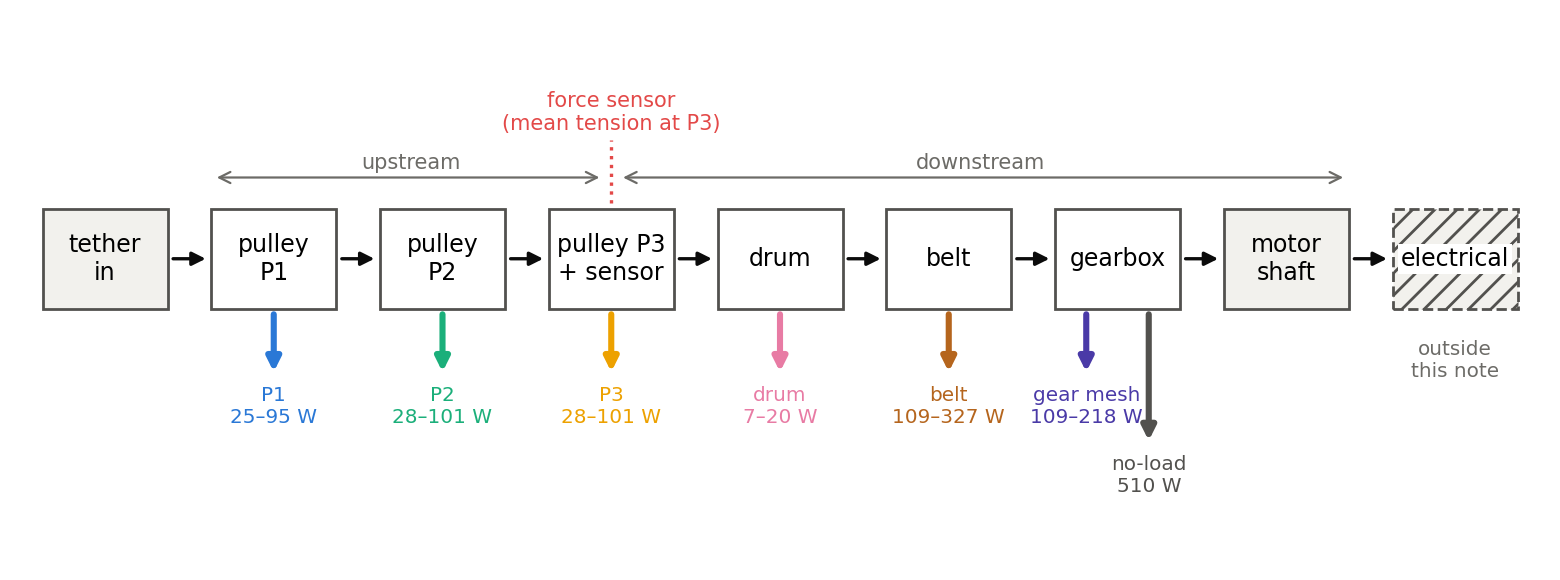
\includegraphics[width=\textwidth]{drivetrain_chain.png}
\caption{The mechanical power chain of GS1 from the tether to the motor shaft,
with the cycle-mean loss of each element on an optimised LEI-V3 cycle
(low--high estimate, Sect.~\ref{sec:est}). The force sensor on P3 splits the
chain into an upstream and a downstream part (Sect.~\ref{sec:sensor}). The
electrical conversion is not part of the estimate.}
\label{fig:chain}
\end{figure}

The tether delivers the power $T v$, with $T$ the tension and $v$ the reel
speed (positive in reel-out). Each element $i$ of the chain in
Fig.~\ref{fig:chain} takes a share of it, so the motor shaft receives
\begin{equation}
  P_\mathrm{shaft} = T v - \sum_i F_i(v, T)\,|v| .
  \label{eq:chain}
\end{equation}
Each loss is written as an equivalent force $F_i \ge 0$ at the tether. This
makes the elements directly comparable, whatever shaft they sit on:
\begin{itemize}
  \item a loss torque $M$ on a shaft of radius $R$ that turns with the tether
    (a pulley, the drum) is $F = M/R$;
  \item a loss torque on the motor side is $F = M\,n/R_\mathrm{drum}$, with $n$
    the overall ratio of belt and gearbox. On GS1, $n = 6.2$ and
    $R_\mathrm{drum} = \SI{0.1615}{m}$, so a modest \SI{1}{N.m} at the motor
    is already \SI{38}{N} at the tether.
\end{itemize}
A loss costs energy in both reel directions. In reel-out it reduces what
reaches the generator; in reel-in the motor supplies it on top of the work done
on the tether.

\paragraph{Three scaling classes.} Every mechanism below falls into one of
three classes (Fig.~\ref{fig:classes}):
\begin{itemize}
  \item \textbf{Constant (Coulomb)}: a fixed force, so the lost power grows
    with $|v|$. Contact seals, bearing preload, belt pretension.
  \item \textbf{Proportional to tension}: $F = k\,T$, a fixed fraction of the
    transmitted power. Bearings under the tether load, rope bending over
    sheaves, belt and gear-mesh friction.
  \item \textbf{Speed-dependent (viscous)}: $F \propto |v|$ or faster, so the
    lost power grows at least as $v^2$. Oil churning, fan windage.
\end{itemize}
The first and third classes do not depend on the load: they are paid in full
even when the transmitted power is small. That is why they dominate the
reel-in, where the tension is low and the speed high.

\begin{figure}[H]
\centering
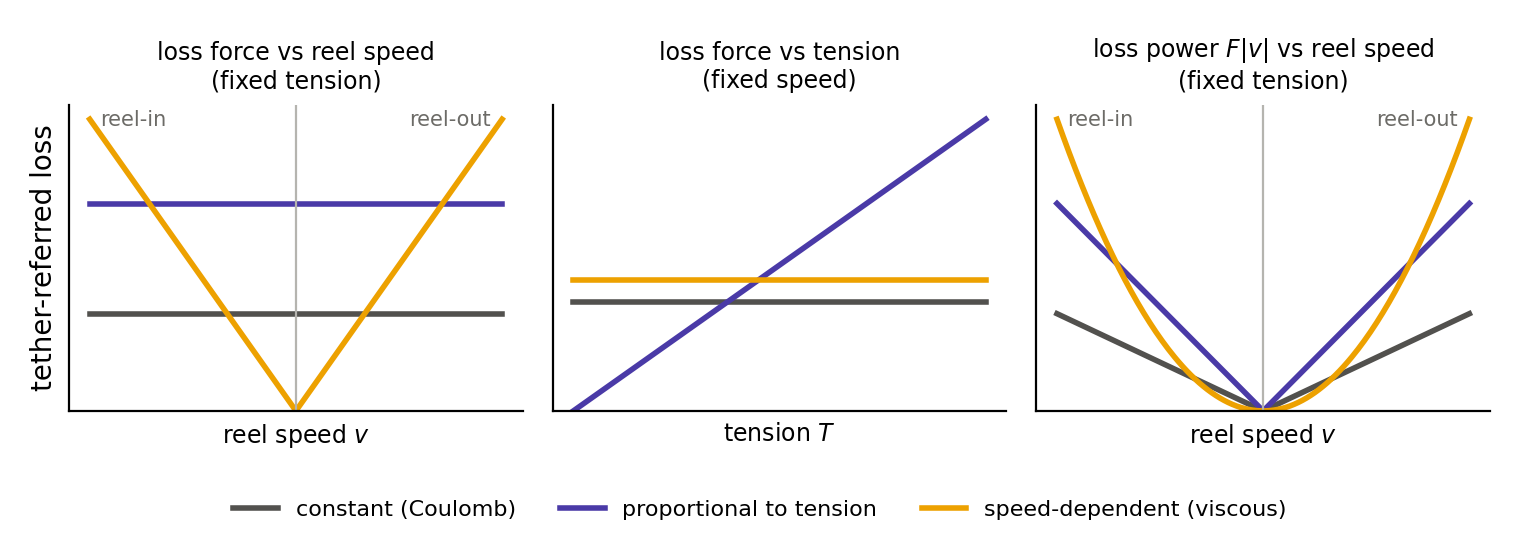
\includegraphics[width=\textwidth]{drivetrain_scaling_classes.png}
\caption{The three loss classes, qualitatively. Left: force against reel
speed. Centre: force against tension. Right: lost power against reel speed.
Only the tension-proportional class shrinks when the load is low.}
\label{fig:classes}
\end{figure}

Inertia (drum, gears, rotor) stores and returns energy and integrates to zero
over a closed cycle. It matters for torque peaks and control, not for the cycle
energy, and is not a loss here.

% ===========================================================================
\section{GS1: tether path and where the force is measured}
\label{sec:sensor}

\begin{figure}[H]
\centering
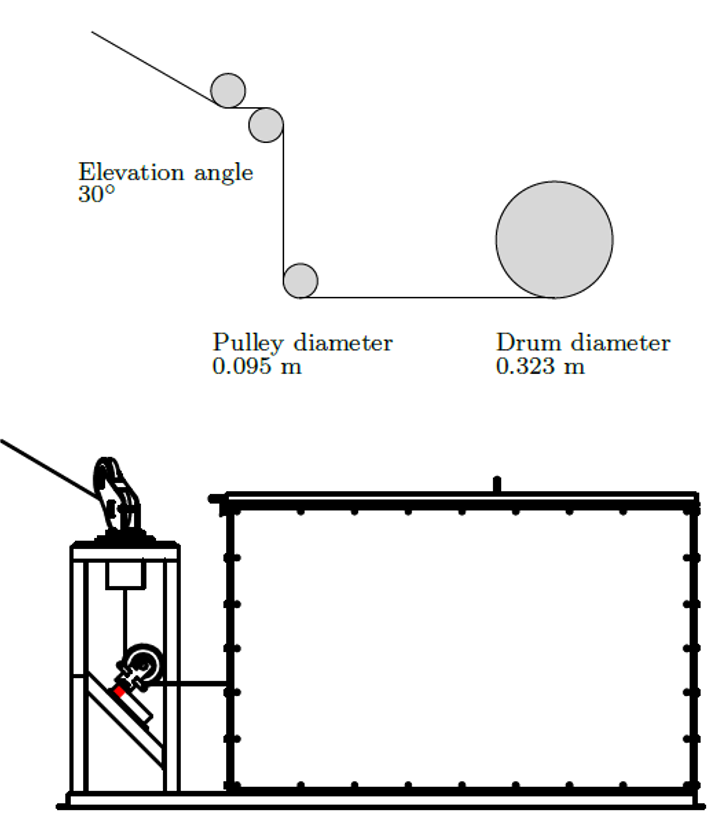
\includegraphics[width=0.62\textwidth]{ground_station_layout.png}
\caption{Tether path of GS1 (schematic above, drawing below). Pulleys P1, P2
and P3 are \SI{0.095}{m} in diameter; the drum is \SI{0.323}{m}. The force
sensor is on the axle of P3, the lowest pulley.}
\label{fig:layout}
\end{figure}

GS1 \cite{fechner2011} had one \SI{18}{kW} motor-generator for both reel
directions, driving the drum through a synchronous belt and a gearbox; three
pulleys with a force sensor; a spindle drive for level winding
(Sect.~\ref{sec:drum}); and a \SI{350}{V} battery. The tether arrives at the
elevation angle $\beta$, turns over P1 by $\beta$ (\ang{30} in the drawing),
over P2 by \ang{90} to vertical, over P3 by \ang{90} to horizontal, and runs
straight onto the drum.

\paragraph{What the sensor reads.}
A pulley axle is loaded by the two rope tensions acting on it
(Fig.~\ref{fig:axle}). With equal tensions and a wrap angle $\theta$ the
resultant is
\begin{equation}
  F_\mathrm{axle} = 2\,T \sin(\theta/2),
  \label{eq:axle}
\end{equation}
so $\sqrt{2}\,T$ on P3. The station's processing converts this axle force to
tether tension, so the logged ground force is already the tension. What
matters here is \emph{which} tension: with friction in P3, the incoming and
outgoing tensions differ by that pulley's loss. The axle resultant is
$\sqrt{T_\mathrm{in}^2 + T_\mathrm{out}^2} \approx \sqrt{2}\,\bar T$, so the
sensor reads the mean tension at P3, and half of P3's loss lies on either side
of the measurement.

\begin{figure}[H]
\centering
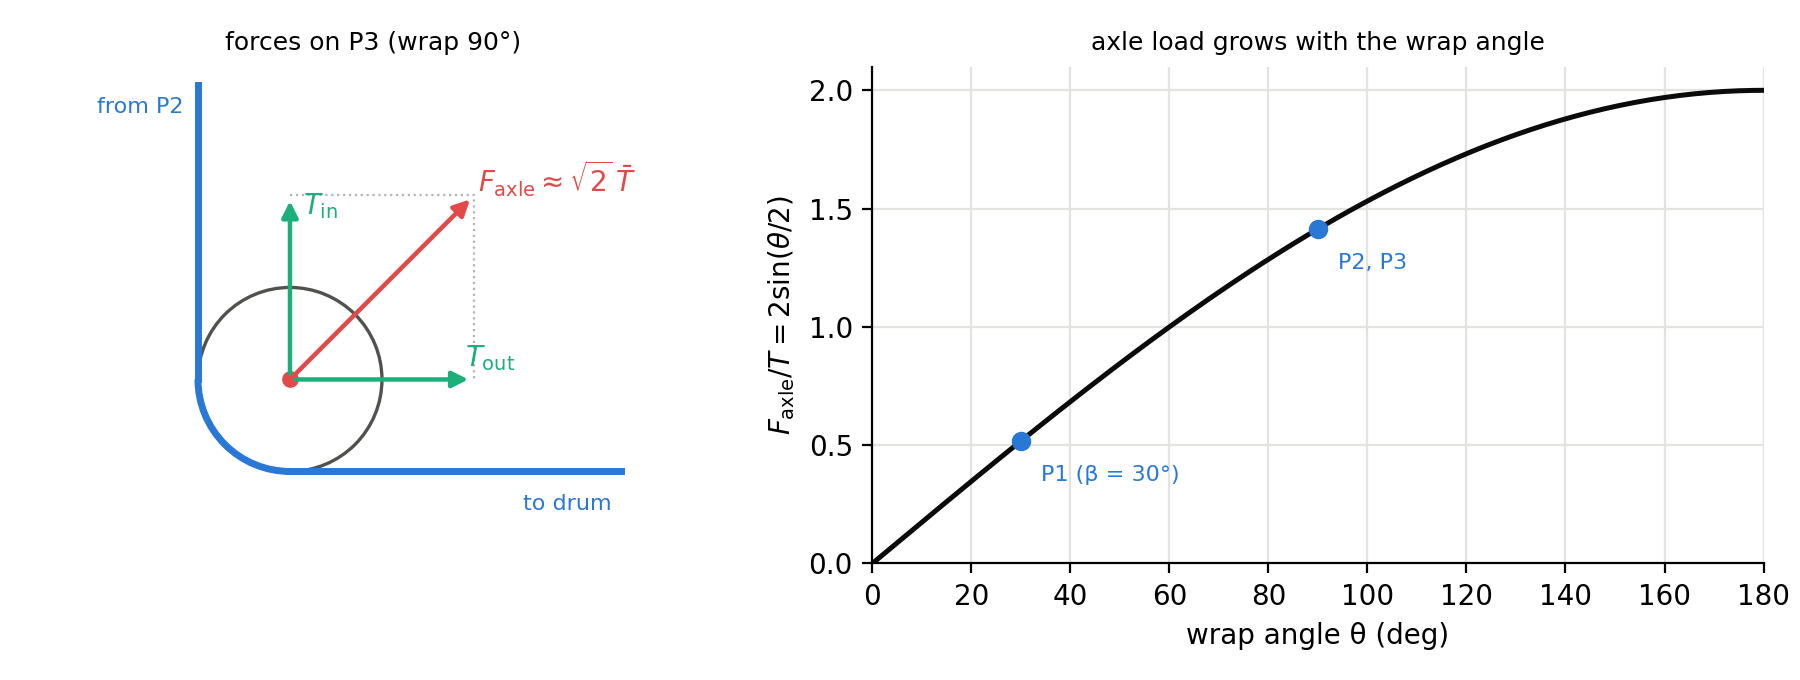
\includegraphics[width=0.92\textwidth]{drivetrain_axle_force.png}
\caption{Left: the two rope tensions on P3 and their resultant, the force the
sensor measures. Right: the axle load relative to the tension against the wrap
angle. It also sets the bearing load of each pulley (Sect.~\ref{sec:pulleys}).}
\label{fig:axle}
\end{figure}

This splits the drivetrain into two parts:
\begin{itemize}
  \item \textbf{Upstream} of the measurement: P1, P2 and half of P3. These
    losses lower the tension before it is measured. A kite model calibrated on
    the measured ground force already absorbs them, and a comparison of sensor
    force with drive power does not see them.
  \item \textbf{Downstream}: half of P3, the drum, the belt, the gearbox and
    the motor's mechanical losses. This is the part a power comparison at the
    sensor measures.
\end{itemize}

% ===========================================================================
\section{Component physics}

\subsection{Pulleys}
\label{sec:pulleys}
A pulley loses power in two ways (Fig.~\ref{fig:pulley}).

\paragraph{Bearing friction.} The sheave turns on rolling bearings that carry
the axle load of Eq.~\eqref{eq:axle}. To first order, the friction torque of a
rolling bearing is $M = \mu_\mathrm{b}\,F_\mathrm{axle}\,d_\mathrm{b}/2$, with
$\mu_\mathrm{b}$ the friction coefficient and $d_\mathrm{b}$ the bore diameter.
Catalogues give $\mu_\mathrm{b} \approx 0.0015$ for deep-groove ball bearings
and slightly more for roller bearings; contact seals add a roughly constant
torque \cite{skf}. Referred to the tether over a sheave of diameter $D$,
\begin{equation}
  F_\mathrm{bearing} = \mu_\mathrm{b}\; 2T\sin(\theta/2)\;\frac{d_\mathrm{b}}{D} .
\end{equation}
It grows with the tension and the wrap angle, but the small lever arm
$d_\mathrm{b}/D$ keeps it at about \SI{0.05}{\percent} of $T$ per pulley.

\paragraph{Bending of the tether.} The larger loss is in the tether itself. A
rope running onto a sheave is bent to the radius $D/2$ and straightened again
when it leaves. In a braided fibre rope such as a Dyneema tether, bending makes
the strands slide against each other under the radial pressure the tension
produces, and the fibres and coating dissipate part of the bending work
(hysteresis). Both grow with the tension and with the curvature $1/D$, so per
bend--unbend cycle
\begin{equation}
  F_\mathrm{bend} \approx c_\mathrm{b}\,\frac{d}{D}\,T ,
\end{equation}
with $d$ the rope diameter and $c_\mathrm{b}$ an empirical coefficient. The
ratio $D/d$ is the main design parameter for both the bending loss and the
bending fatigue of ropes \cite{feyrer}. Each sheave costs one full cycle,
whatever its wrap angle, as long as the rope conforms to the groove. With a
\SI{4}{mm} tether, $D/d = 24$; a coefficient of 0.05--0.2 gives
\SIrange{0.2}{0.8}{\percent} of the tension per pulley, the typical sheave
efficiency range for fibre rope. This is the dominant pulley loss and the most
uncertain pulley parameter.

\begin{figure}[H]
\centering
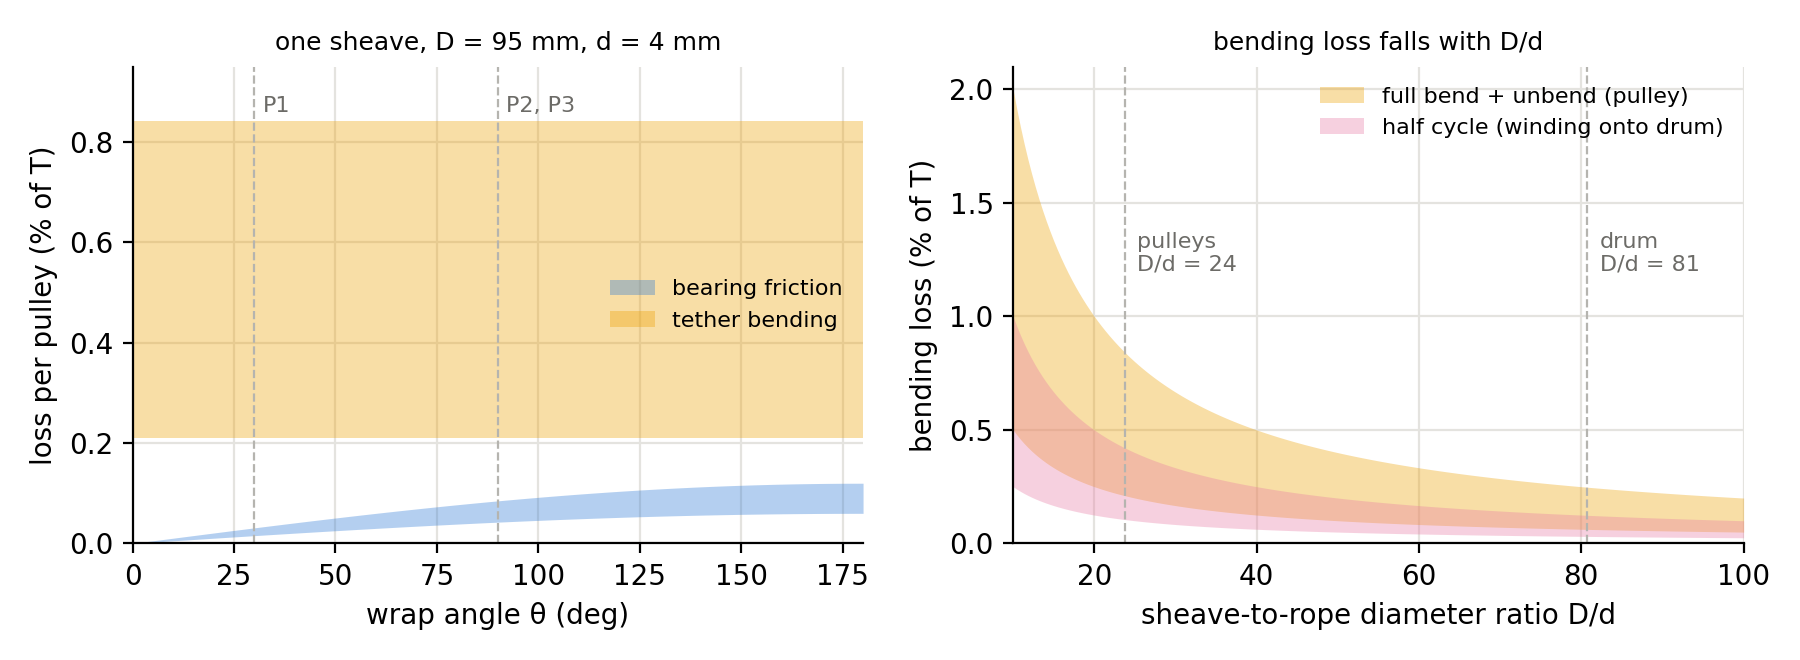
\includegraphics[width=0.95\textwidth]{drivetrain_pulley_physics.png}
\caption{Left: loss of one GS1 pulley as a fraction of the tension, bearing
friction against tether bending (bands = assumed parameter range). Bending
dominates and does not depend on the wrap angle. Right: the bending loss falls
as $d/D$; the drum, with a larger diameter and only half a cycle per pass,
loses far less than a pulley.}
\label{fig:pulley}
\end{figure}

\subsection{Drum and level winding}
\label{sec:drum}
\begin{itemize}
  \item \textbf{Bending onto the drum.} The tether is bent once when it winds
    on and straightened only when it pays out again: half a cycle per pass, at
    $D/d = 81$. Far smaller than on a pulley (Fig.~\ref{fig:pulley}, right).
  \item \textbf{Drum bearings.} They carry roughly the tension plus the drum's
    weight. With journals of about a fifth of the drum diameter they cost
    $\mu_\mathrm{b} T\,d_\mathrm{b}/D$, a few hundredths of a percent.
  \item \textbf{Spooling.} With several layers, the rope presses into the
    layers below and rubs at the cross-overs.
  \item \textbf{Level winding.} To lay the layers evenly, the tether must move
    along the drum axis by one tether diameter per drum revolution and reverse
    at the drum ends. On GS1 this was done the other way round: the tether exit
    stayed fixed and a spindle motor, through a gearbox and a worm drive,
    moved the drum \emph{together with the generator} back and forth
    \cite{fechner2011}. That moves the heaviest parts of the station instead of
    a light guide pulley. It costs electrical power (200--\SI{600}{W} on GS1,
    Sect.~\ref{sec:gs1}) rather than drum torque, so it is an auxiliary load,
    outside the mechanical chain estimated here. Later stations solved this.
\end{itemize}

\subsection{Belt}
GS1 coupled the drum to the gearbox through a synchronous (toothed) belt. The
teeth slide slightly as they engage and leave the pulley grooves, and the belt
is bent around both pulleys under load; both losses are proportional to the
transmitted force. Toothed belts reach 97--\SI{99}{\percent}, so
$F_\mathrm{belt} = (1-\eta_\mathrm{belt})\,T$, 1--\SI{3}{\percent} of the
tension. The belt pretension adds bearing load and a constant drag, which is
part of the load-independent term.

\subsection{Gearbox}
Gearbox losses are conventionally split into load-dependent and
load-independent parts \cite{iso14179}:
\begin{itemize}
  \item \textbf{Mesh friction} (load-dependent). The tooth flanks slide under
    the transmitted load. A gear stage reaches a mesh efficiency of about
    98--99\,\%, so $F_\mathrm{mesh} = (1-\eta_\mathrm{mesh})\,T$, about
    1--2\,\% of the tension.
  \item \textbf{Bearings} (mostly load-dependent), as for the pulleys.
  \item \textbf{Oil churning and splashing} (speed-dependent). Gears move
    through the oil bath. The loss grows with speed and with the oil viscosity,
    and so depends strongly on the oil temperature (Sect.~\ref{sec:tow}).
    Over-filling raises it.
  \item \textbf{Shaft seals} (constant). Lip seals have a nearly constant
    friction torque, higher when cold.
\end{itemize}

\subsection{Motor, mechanical part}
Before the conversion to electrical power, the motor contributes rotor bearing
friction (constant plus load-dependent) and, for a self-ventilated motor, fan
windage, whose torque grows roughly with the square of the speed. Motor
standards report these together as the friction and windage loss
\cite{iec60034}. They act at motor speed, so the ratio $n$ amplifies them at
the tether.

\subsection{Summary of mechanisms}

\begin{table}[H]
\centering\small
\caption{Mechanical loss mechanisms between the tether and the motor shaft of
GS1.}
\label{tab:mechanisms}
\begin{tabularx}{\textwidth}{lXll}
\toprule
Element & Mechanism & Scaling & Side of sensor \\
\midrule
P1, P2 & bearing friction; tether bending (strand friction, hysteresis) & $\propto T$ & upstream \\
P3 & as P1, P2 & $\propto T$ & half / half \\
Drum & winding bend (half cycle); bearings; spooling & $\propto T$ & downstream \\
Belt & tooth engagement; bending & $\propto T$ & downstream \\
Gearbox & mesh friction; bearings & $\propto T$ & downstream \\
Gearbox & oil churning & $\propto v$ or faster & downstream \\
Belt, gearbox, motor & pretension; seals; bearing preload & constant & downstream \\
Motor & fan windage & $\propto v^2$ (force) & downstream \\
\bottomrule
\end{tabularx}
\end{table}

The two-parameter law used in AWETrim's optimiser,
$F = F_\mathrm{c} + c_v |v|$ \cite{fechner2016}, describes the
load-independent part only: the constant terms and a linearised speed term.
The tension-proportional part (pulleys, drum, belt, gear mesh) is not in it.

% ===========================================================================
\section{Estimate for GS1 on optimised LEI-V3 cycles}
\label{sec:est}

\subsection{Inputs}
The load comes from AWETrim's optimised pumping cycles for the LEI-V3 kite. It
is a \emph{hypothetical} load for GS1: the station was rated for a maximum
tether force of \SI{4000}{N} \cite[Table~3.1]{fechner2016}, while these cycles
reel out at about \SI{7.4}{kN}, nearly twice that; the speeds (up to
\SI{8}{m.s^{-1}} both ways) are within its limits. The tension-proportional
losses scale with the load and keep their share of the power. The
load-independent friction does not, so at GS1's real tensions it would take a
larger share than the estimate below shows.

\begin{table}[H]
\centering\small
\caption{Inputs of the estimate. Known values are GS1's; ranges are typical
values for the element type, not measurements.}
\label{tab:inputs}
\begin{tabular}{llr}
\toprule
Quantity & Value & Status \\
\midrule
Pulley diameter $D$ (P1--P3) & \SI{0.095}{m} & known (drawing) \\
Wrap angles P1 / P2 / P3 & $\beta$ (\ang{30}) / \ang{90} / \ang{90} & known (drawing) \\
Drum diameter & \SI{0.323}{m} & known (drawing) \\
Tether & \SI{4}{mm} braided Dyneema & known \\
Overall ratio $n$ & 6.2 (belt + gearbox) & known \cite{fechner2016} \\
Maximum tether force & \SI{4000}{N} & known \cite{fechner2016} \\
Maximum reel speed, in / out & 8 / \SI{8}{m.s^{-1}} & known \cite{fechner2016} \\
Bearing friction $\mu_\mathrm{b}$ & 0.0015--0.003 & assumed \\
Bore-to-diameter ratio $d_\mathrm{b}/D$ & 0.2 & assumed \\
Bending coefficient $c_\mathrm{b}$ & 0.05--0.2 & assumed \\
Belt loss $1-\eta_\mathrm{belt}$ & 0.01--0.03 & assumed \\
Mesh loss $1-\eta_\mathrm{mesh}$ & 0.01--0.02 & assumed \\
Load-independent $F_\mathrm{c}$ / $c_v$ & \SI{122}{N} / \SI{30.7}{N.s.m^{-1}} & measured (tow test) \\
\bottomrule
\end{tabular}
\end{table}

The load-independent part cannot be estimated reliably from first principles,
because it depends on oil, seals and motor size. It comes from GS1's tow test
(Sect.~\ref{sec:tow}): $\tau_\mathrm{s} = \SI{3.18}{N.m}$ and
$c_\mathrm{f} = \SI{0.799}{N.m.s.m^{-1}}$ on the motor side \cite{fechner2016},
which with $n = 6.2$ and $R_\mathrm{drum} = \SI{0.1615}{m}$ is
\SI{122}{N} + \SI{30.7}{N.s.m^{-1}}\,$|v|$ at the tether. It is one measured
value, so it carries no low--high range here; its own bias (a cold gearbox) is
discussed in Sect.~\ref{sec:tow}. The low--high ranges below come from the
load-dependent parameters only.

\subsection{Loss by component}

\begin{figure}[H]
\centering
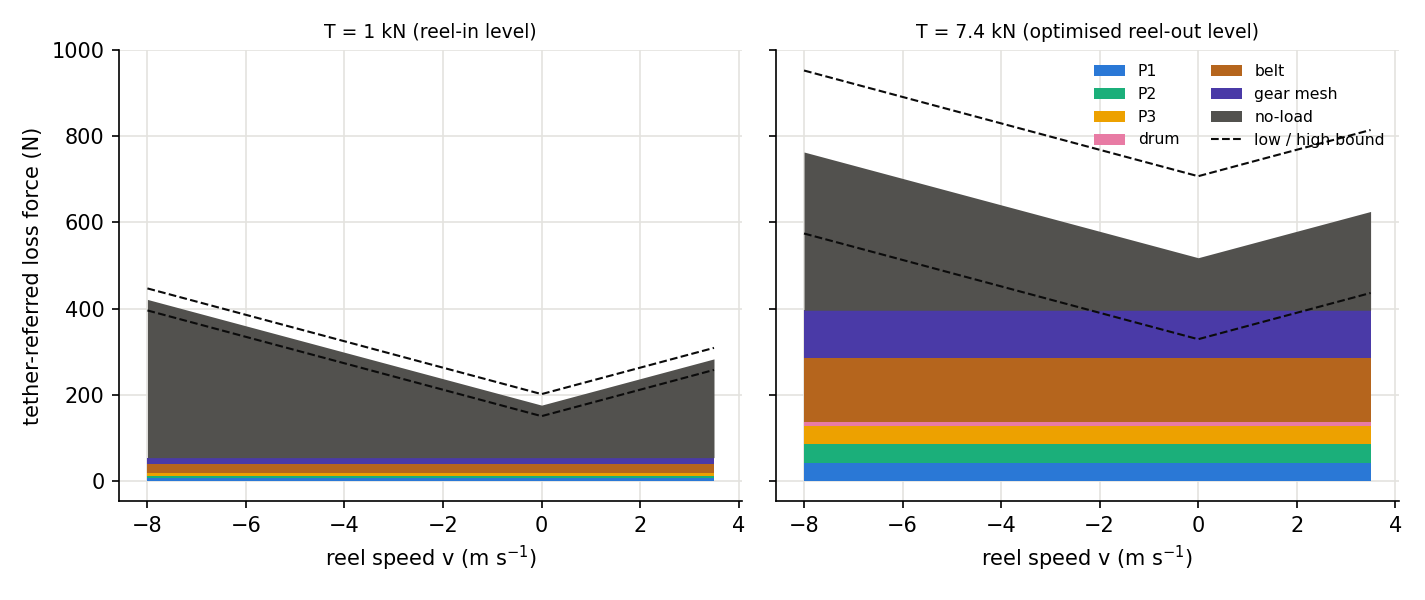
\includegraphics[width=\textwidth]{drivetrain_breakdown.png}
\caption{Tether-referred loss force by component against reel speed, at a
reel-in tension (left) and an optimised reel-out tension (right). Coloured
areas stack the mid-range estimates; the dashed lines are the low and high
totals.}
\label{fig:breakdown}
\end{figure}

\begin{table}[H]
\centering\scriptsize
\setlength{\tabcolsep}{3pt}
\caption{Loss force by component (N, low--high) at representative operating
points. ``Upstream'' and ``downstream'' are relative to the force sensor on P3.}
\label{tab:points}
\resizebox{\textwidth}{!}{\begin{tabular}{lrrrrrrrrrr}
\toprule
Operating point & P1 & P2 & P3 & drum & belt & gear mesh & no-load & upstream & downstream & total \\
\midrule
Moderate reel-out (2.8~kN, +1.10~m\,s$^{-1}$) & 6--24 & 7--26 & 7--26 & 2--5 & 28--84 & 28--56 & 156 & 17--63 & 217--314 & 234--377 \\
Optimised reel-out (7.4~kN, +1.75~m\,s$^{-1}$) & 17--65 & 19--69 & 19--69 & 5--14 & 74--222 & 74--148 & 176 & 45--168 & 338--594 & 382--761 \\
Typical reel-in (1.0~kN, -3.50~m\,s$^{-1}$) & 2--9 & 3--9 & 3--9 & 1--2 & 10--30 & 10--20 & 229 & 6--23 & 251--286 & 257--309 \\
Fast reel-in (1.0~kN, -8.00~m\,s$^{-1}$) & 2--9 & 3--9 & 3--9 & 1--2 & 10--30 & 10--20 & 368 & 6--23 & 389--424 & 396--447 \\
\bottomrule
\end{tabular}
}
\end{table}

\begin{itemize}
  \item \textbf{At low tension}, as in reel-in, the load-independent friction
    is almost the entire loss, and it grows with the reel speed.
  \item \textbf{At high tension}, as in optimised reel-out, the
    tension-proportional elements become visible. At \SI{7.4}{kN}: the belt
    \SIrange{\roBeltLow}{\roBeltHigh}{N}, the gear mesh
    \SIrange{\roMeshLow}{\roMeshHigh}{N}, the three pulleys together
    \SIrange{\roPulleyLow}{\roPulleyHigh}{N}, against \SI{176}{N} of
    load-independent friction. The drum costs a few newtons.
  \item \textbf{P1's loss barely depends on elevation}: its bending loss is
    independent of the wrap, and only its small bearing term follows
    $\sin(\beta/2)$.
\end{itemize}

\subsection{Efficiency map}
Dividing the losses by the transmitted power gives the mechanical efficiency
at every operating point (Fig.~\ref{fig:effmap}). In reel-out it is shaft over
tether power; in reel-in, where the motor drives, tether over shaft power. The
map shows the consequence of the scaling classes: at high tension the fixed
friction is small next to the transmitted power and the efficiency is around
\SI{90}{\percent}; at low tension and high speed it falls well below. The
optimised cycle spends its reel-out in the good corner and its reel-in in the
poor one.

\begin{figure}[H]
\centering
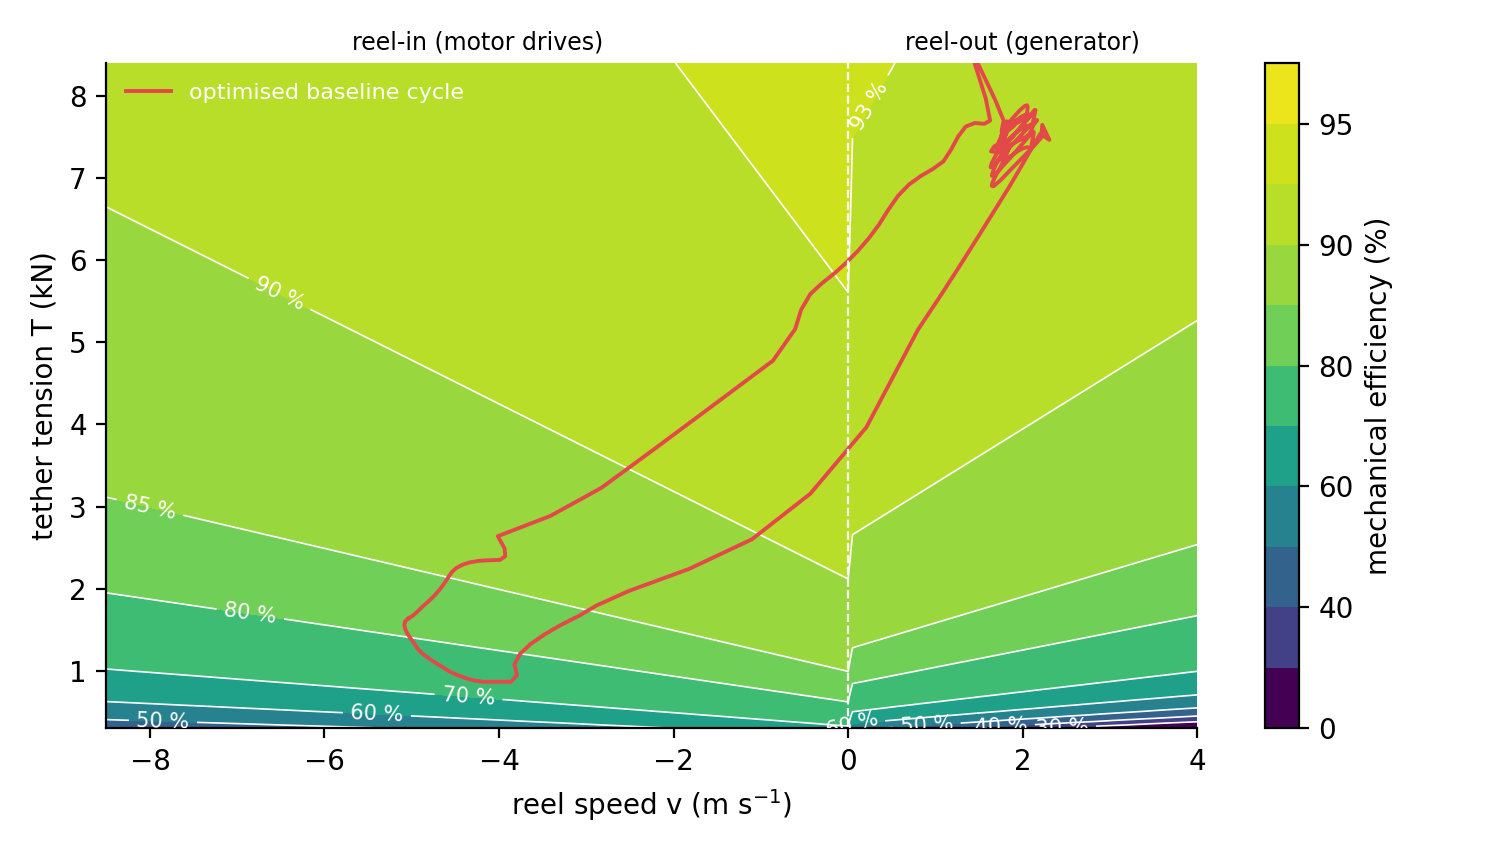
\includegraphics[width=0.85\textwidth]{drivetrain_efficiency_map.png}
\caption{Mechanical drivetrain efficiency of GS1 (mid-range estimate) against
reel speed and tension, with the optimised LEI-V3 baseline cycle overlaid.}
\label{fig:effmap}
\end{figure}

\subsection{Over a pumping cycle}
\label{sec:cycle}
Figure~\ref{fig:timeseries} shows the optimised LEI-V3 baseline cycle
(logarithmic wind \SI{10}{m.s^{-1}} at \SI{100}{m}, tether power
\SI{\cyclePtether}{kW}) with the loss power of each element over time.

\begin{figure}[H]
\centering
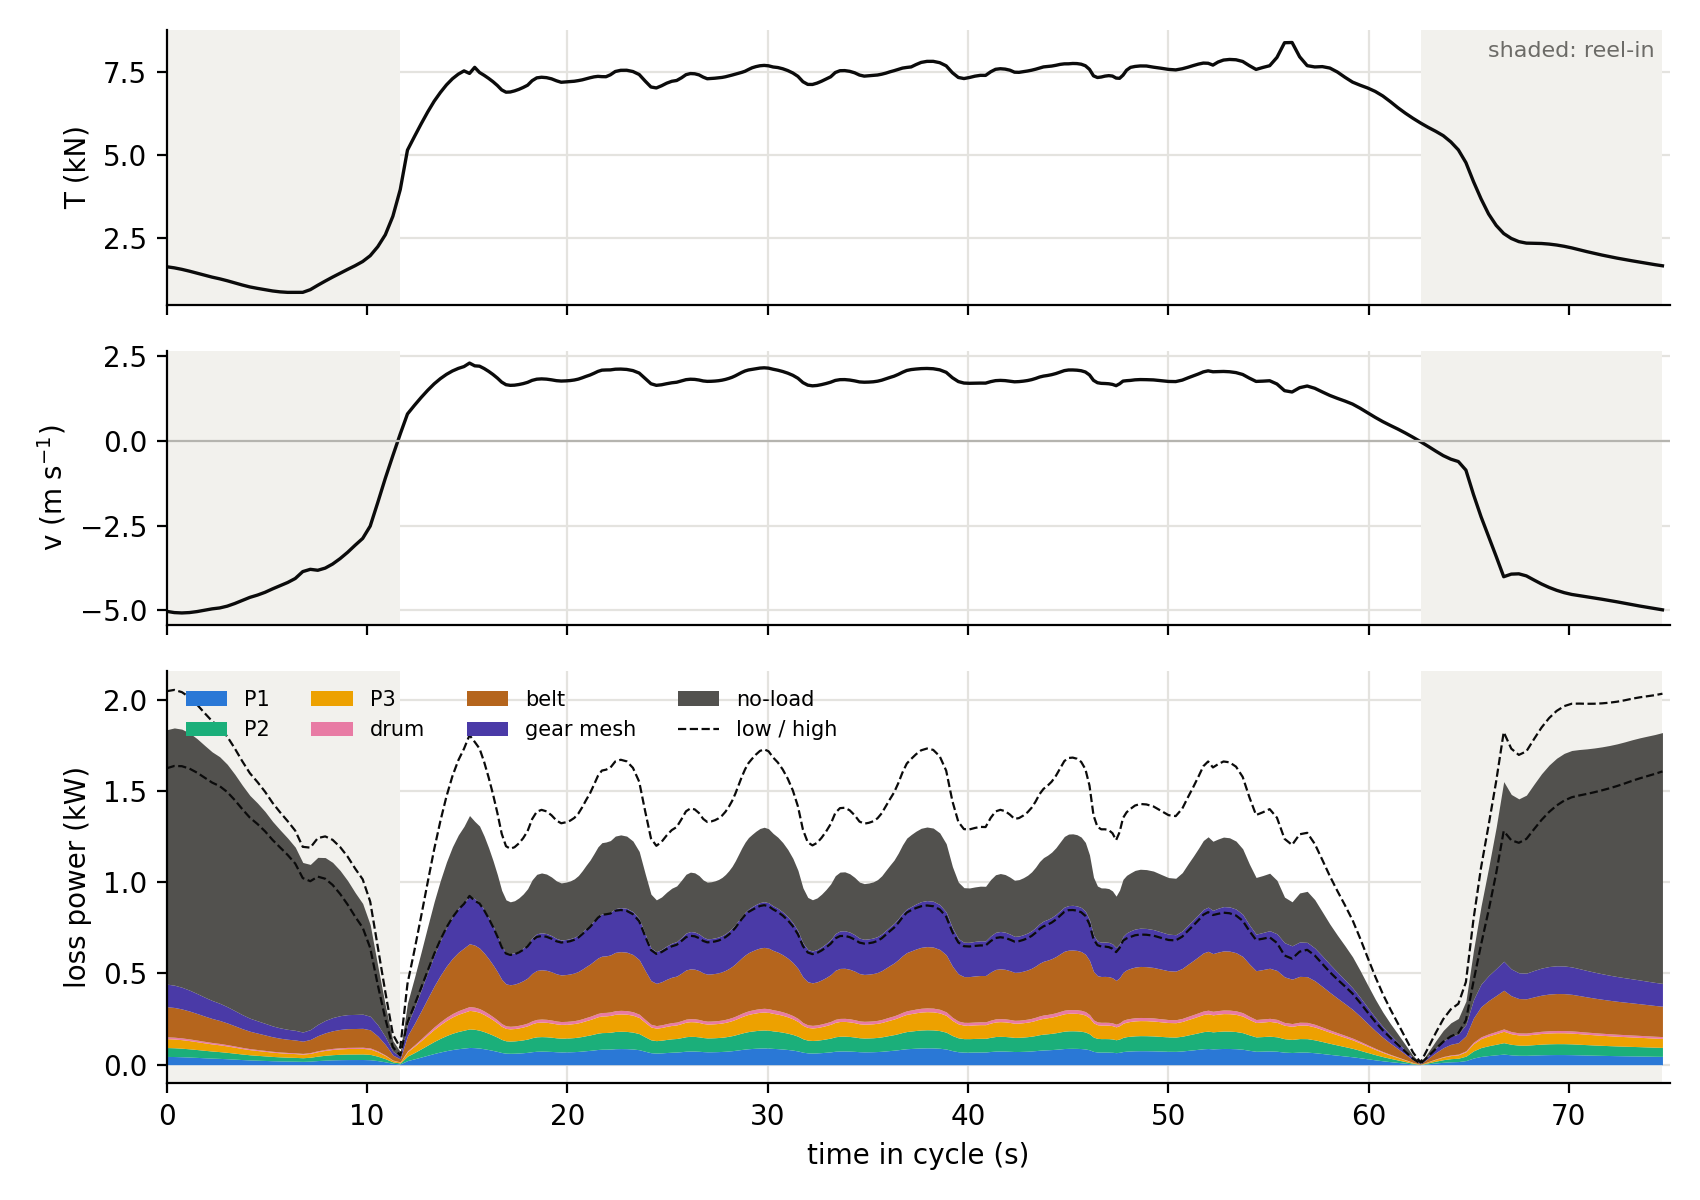
\includegraphics[width=0.9\textwidth]{drivetrain_cycle_timeseries.png}
\caption{Tension, reel speed and mechanical loss power over the optimised
baseline cycle. The stacked areas are the mid-range estimate per component,
the dashed lines the low and high totals; reel-in is shaded.}
\label{fig:timeseries}
\end{figure}

\begin{figure}[H]
\centering
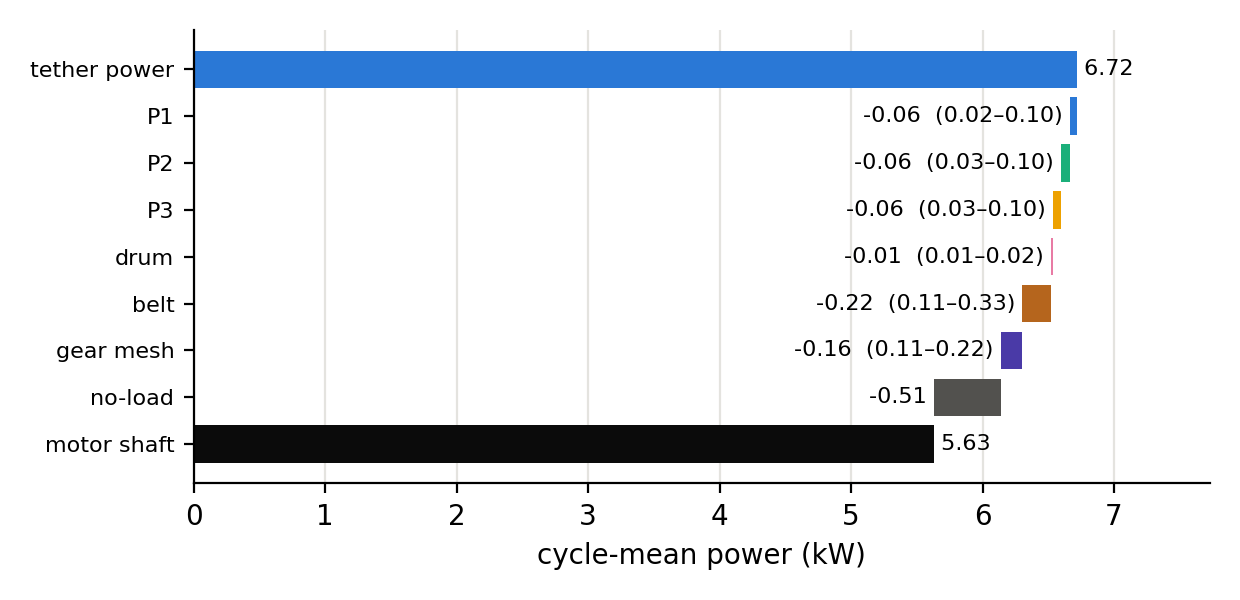
\includegraphics[width=0.8\textwidth]{drivetrain_cycle_waterfall.png}
\caption{Cycle-mean power from the tether to the motor shaft on the baseline
cycle: mid-range loss per element, low--high in brackets (kW).}
\label{fig:waterfall}
\end{figure}

\begin{table}[H]
\centering\scriptsize
\setlength{\tabcolsep}{3pt}
\caption{Share of the cycle's tether energy lost per component (low--high).}
\label{tab:cycle}
\resizebox{\textwidth}{!}{\begin{tabular}{lrrrrrrrrrr}
\toprule
 & P1 & P2 & P3 & drum & belt & gear mesh & no-load & upstream & downstream & total \\
\midrule
mean loss power (W) & 25--95 & 28--101 & 28--101 & 7--20 & 109--327 & 109--218 & 510 & 66--246 & 748--1125 & 814--1371 \\
share of $\int T v\,\mathrm{d}t$ (\%) & 0.4--1.4 & 0.4--1.5 & 0.4--1.5 & 0.1--0.3 & 1.6--4.9 & 1.6--3.2 & 7.6 & 1.0--3.7 & 11.1--16.7 & 12.1--20.4 \\
\bottomrule
\end{tabular}
}
\end{table}

\begin{itemize}
  \item \textbf{Total.} The mechanical losses take
    \SIrange{\cycleLossLow}{\cycleLossHigh}{\percent} of the tether energy, of
    which \SIrange{\cycleDownLow}{\cycleDownHigh}{\percent} is downstream of
    the sensor.
  \item \textbf{The load-independent friction} takes
    \SI{\cycleNoLoadLow}{\percent}, the largest single item.
  \item \textbf{Belt} \SIrange{\cycleBeltLow}{\cycleBeltHigh}{\percent},
    \textbf{gear mesh} \SIrange{\cycleMeshLow}{\cycleMeshHigh}{\percent},
    \textbf{the three pulleys} together
    \SIrange{\cyclePulleyLow}{\cyclePulleyHigh}{\percent} (mostly upstream of
    the sensor), \textbf{the drum} almost nothing.
  \item \textbf{Peaks of \SIrange{\peakLow}{\peakHigh}{kW}} occur at the
    fast start of the reel-in and in the reel-out (Fig.~\ref{fig:timeseries}).
\end{itemize}

\subsection{Power loss at operating points and across cycles}
The loss power of each element is its force times the reel speed,
$P_i = F_i\,|v|$ (Table~\ref{tab:power}).

\begin{table}[H]
\centering\scriptsize
\setlength{\tabcolsep}{3pt}
\caption{Loss power by component (W, low--high) at the operating points of
Table~\ref{tab:points}.}
\label{tab:power}
\resizebox{\textwidth}{!}{\begin{tabular}{lrrrrrrrrrr}
\toprule
Operating point & P1 & P2 & P3 & drum & belt & gear mesh & no-load & upstream & downstream & total \\
\midrule
Moderate reel-out (2.8~kN, +1.10~m\,s$^{-1}$) & 7--27 & 8--29 & 8--29 & 2--6 & 31--92 & 31--62 & 171 & 19--70 & 239--345 & 257--415 \\
Optimised reel-out (7.4~kN, +1.75~m\,s$^{-1}$) & 29--113 & 33--120 & 33--120 & 8--24 & 130--388 & 130--259 & 308 & 78--293 & 591--1039 & 669--1332 \\
Typical reel-in (1.0~kN, -3.50~m\,s$^{-1}$) & 8--31 & 9--32 & 9--32 & 2--6 & 35--105 & 35--70 & 803 & 21--79 & 880--1001 & 901--1080 \\
Fast reel-in (1.0~kN, -8.00~m\,s$^{-1}$) & 18--70 & 20--74 & 20--74 & 5--15 & 80--240 & 80--160 & 2941 & 48--181 & 3116--3393 & 3164--3574 \\
\bottomrule
\end{tabular}
}
\end{table}

\begin{itemize}
  \item \textbf{Reel-out.} At \SI{7.4}{kN} and \SI{1.75}{m.s^{-1}}
    (\SI{13}{kW} at the tether) the drivetrain takes
    \SIrange{\roLossLow}{\roLossHigh}{kW}, or
    \SIrange{\roPctLow}{\roPctHigh}{\percent}.
  \item \textbf{Reel-in.} At \SI{3.5}{m.s^{-1}} and \SI{1}{kN} the tether
    absorbs \SI{3.5}{kW} and the drivetrain adds
    \SIrange{\riLossLow}{\riLossHigh}{kW}.
  \item \textbf{Fast reel-in.} At \SI{8}{m.s^{-1}} the drivetrain adds
    \SIrange{\rfLossLow}{\rfLossHigh}{kW}, about \SI{40}{\percent} on top of
    the \SI{8}{kW} the tether absorbs.
\end{itemize}

\begin{table}[H]
\centering\scriptsize
\caption{Cycle-mean mechanical loss power of GS1 on the optimised LEI-V3
cycles (low--high). ``Shaft'' is the mean power at the motor shaft, tether
power minus the loss.}
\label{tab:cycles}
\resizebox{\textwidth}{!}{\begin{tabular}{lrrrrrr}
\toprule
Cycle & tether (kW) & loss (kW) & loss (\%) & shaft (kW) & reel-in share of loss (\%) & peak loss (kW) \\
\midrule
baseline (multi-lobe) (75~s) & 6.72 & 0.81--1.37 & 12.1--20.4 & 5.35--5.91 & 34--44 & 1.6--2.1 \\
up-loop eight (74~s) & 6.06 & 0.76--1.27 & 12.5--20.9 & 4.79--5.30 & 34--43 & 1.4--1.9 \\
symmetric eight (57~s) & 4.63 & 0.59--1.04 & 12.7--22.4 & 3.59--4.04 & 33--41 & 0.9--1.8 \\
symmetric eight, mirrored (79~s) & 4.76 & 0.63--1.08 & 13.2--22.7 & 3.68--4.13 & 34--42 & 1.0--1.8 \\
\bottomrule
\end{tabular}
}
\end{table}

Across the four optimised cycles (Table~\ref{tab:cycles}) the drivetrain takes
\SIrange{\allLossKWLow}{\allLossKWHigh}{kW} of 4.6--\SI{6.7}{kW}, so the shaft
receives \SIrange{\shaftShareLow}{\shaftShareHigh}{\percent} of the tether
power. The reel-in carries
\allReelinShareLow--\SI{\allReelinShareHigh}{\percent} of the loss although it
lasts only about a third of the cycle, because it runs about twice as fast as
the reel-out. The percentage hardly depends on the cycle shape
(\SIrange{\allPctLow}{\allPctHigh}{\percent}), so the drivetrain lowers all
cycles by a similar factor and does not change their ranking.

\subsection{Optimising for shaft power instead of tether power}
\label{sec:objective}
The cycles above were optimised for the cycle-mean \emph{tether} power $T v$
and the drive losses were evaluated afterwards. AWETrim's optimiser can instead
maximise the cycle-mean \emph{shaft} power, the tether power minus the drive
losses of this section, written in the same tether-referred form:
\begin{equation}
  P_\mathrm{shaft} = T v - \left(F_\mathrm{c} + k\,T\right) v \tanh(v/\varepsilon)
  - c_v v^2 ,
\end{equation}
with the GS1 tow-test friction ($F_\mathrm{c} = \SI{122}{N}$,
$c_v = \SI{30.7}{N.s.m^{-1}}$), the tension-proportional fraction
$k = 0.0535$ of the mid estimate (pulleys, drum, belt, gear mesh; range
0.028--0.079) and $\varepsilon = \SI{0.05}{m.s^{-1}}$ smoothing the sign of
$v$ (\code{sim\_parameters.winch\_friction} and
\code{drivetrain\_load\_fraction}). Table~\ref{tab:objectives} compares the
optima of the two objectives on the multi-lobe baseline and the up-loop eight.

\begin{table}[H]
\centering\scriptsize
\setlength{\tabcolsep}{3pt}
\caption{Optima of the tether-power and shaft-power objectives, both evaluated
for tether and shaft power (mid estimate, low--high in brackets). Barred
values are time means over the reel-out (out) and the reel-in (in).}
\label{tab:objectives}
\resizebox{\textwidth}{!}{\begin{tabular}{llrrrrrrrr}
\toprule
Cycle & objective & period & tether & shaft & reel-in & $\bar v_\mathrm{out}$ & $\bar T_\mathrm{out}$ & $\bar v_\mathrm{in}$ & $\bar T_\mathrm{in}$ \\
 & & (s) & (kW) & (kW) & time (\%) & (m\,s$^{-1}$) & (kN) & (m\,s$^{-1}$) & (kN) \\
\midrule
baseline (multi-lobe) & tether power $Tv$ & 75 & 6.72 & 5.63 (5.35--5.91) & 32 & 1.74 & 7.38 & 3.67 & 2.22 \\
baseline (multi-lobe) & shaft power, from the $Tv$ optimum & 79 & 6.68 & 5.66 (5.39--5.92) & 32 & 1.64 & 7.54 & 3.50 & 2.07 \\
baseline (multi-lobe) & shaft power, from the seed & 66 & 6.28 & 5.31 (5.05--5.57) & 31 & 1.49 & 7.95 & 3.33 & 2.33 \\
up-loop eight & tether power $Tv$ & 74 & 6.06 & 5.04 (4.79--5.30) & 37 & 1.82 & 6.82 & 3.09 & 2.17 \\
up-loop eight & shaft power, from the seed & 69 & 6.00 & 5.10 (4.86--5.33) & 36 & 1.63 & 7.01 & 2.90 & 1.68 \\
\bottomrule
\end{tabular}
}
\end{table}

\begin{figure}[H]
\centering
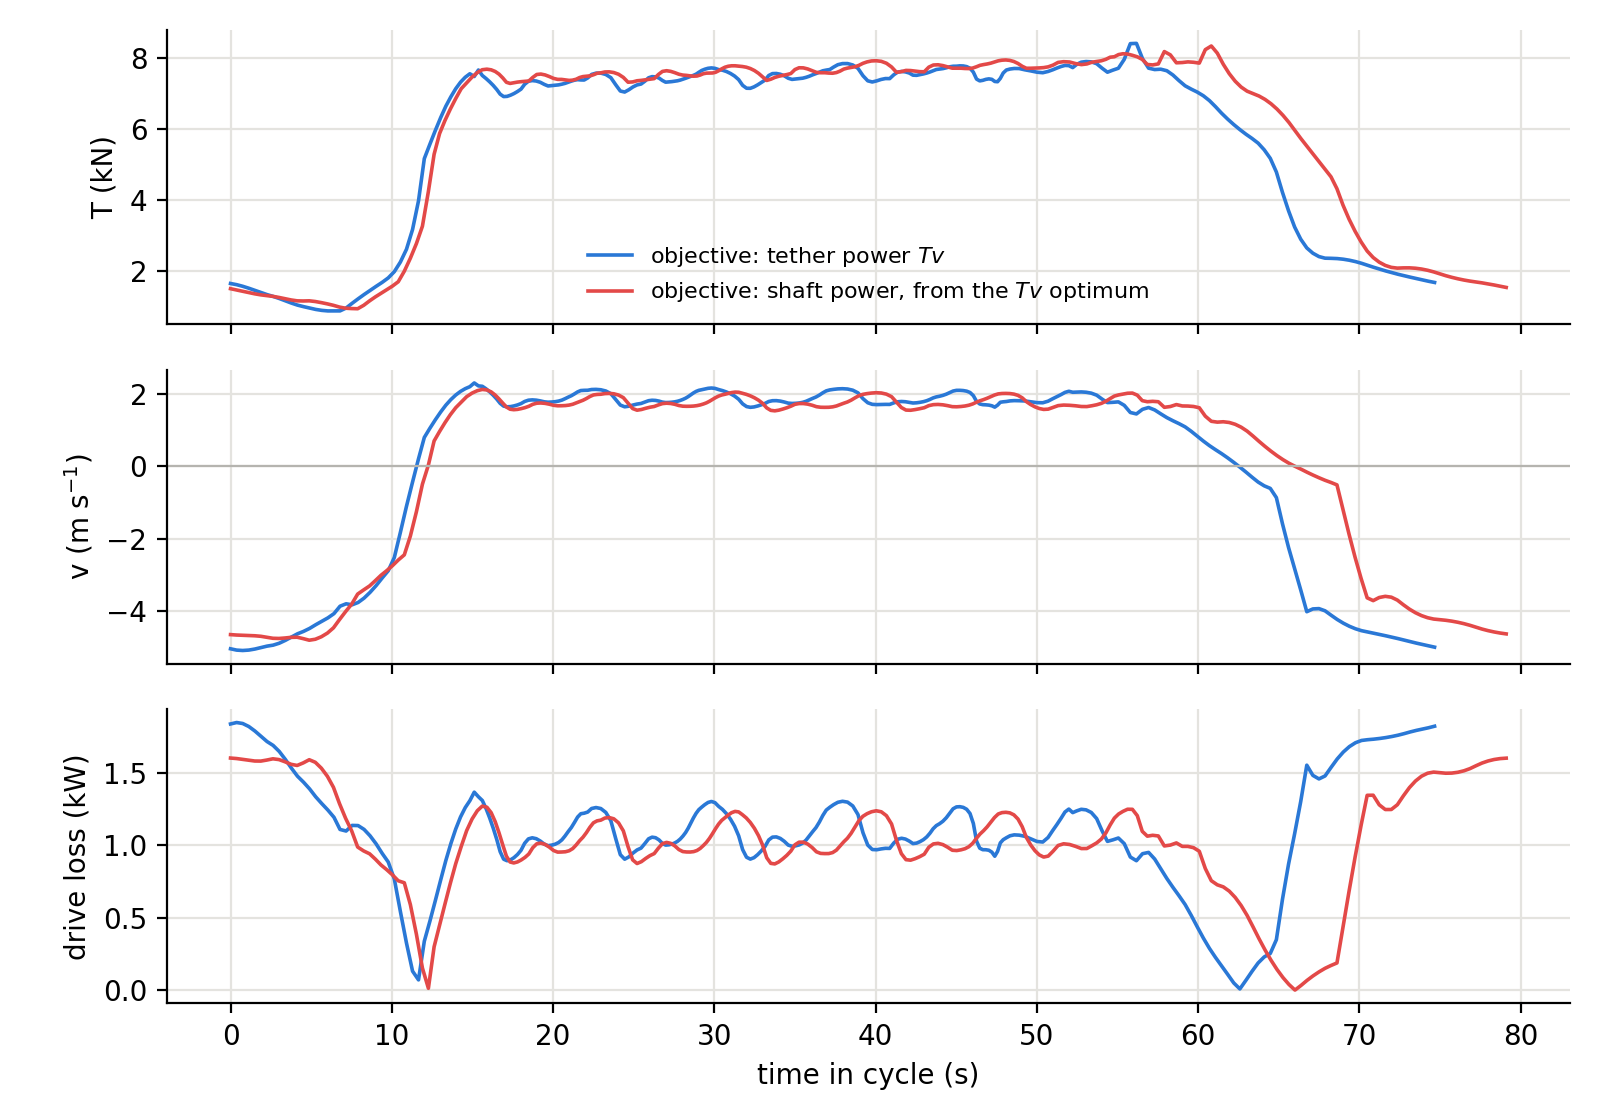
\includegraphics[width=0.85\textwidth]{drivetrain_objectives.png}
\caption{Multi-lobe baseline: tension, reel speed and drive loss over the cycle
for the tether-power optimum (blue) and the shaft-power optimum started from it
(red).}
\label{fig:objectives}
\end{figure}

\begin{itemize}
  \item \textbf{The gain is small.} Started from the tether-power optimum, the
    shaft-power optimum of the baseline delivers \SI{\objShaftB}{kW} at the
    shaft instead of \SI{\objShaftA}{kW} (\objShaftGainB\,\%), for
    \objTetherChangeB\,\% tether power. The up-loop eight gains
    \objShaftGainF\,\%. The optimum is flat: the drive loss is mostly a cost
    of the hardware, not of the way the cycle is flown.
  \item \textbf{The strategy moves the way the loss classes predict.} The
    reel-in becomes slower (mean \SI{\objVinA}{} $\to$
    \SI{\objVinB}{m.s^{-1}}, peak \SI{\objVinMaxA}{} $\to$
    \SI{\objVinMaxB}{m.s^{-1}} on the baseline; \SI{\objVinE}{} $\to$
    \SI{\objVinF}{m.s^{-1}} on the eight) and is flown at lower tension, so the
    reel-in tether work drops by \objEinChangeB\,\% and \objEinChangeF\,\%. The
    reel-out becomes slower and stronger (\SI{\objToutA}{} $\to$
    \SI{\objToutB}{kN}). Both changes cut the speed-dependent friction; the
    tension-proportional loss is a fixed fraction of the power and does not
    favour either.
  \item \textbf{A fast reel-in still pays.} The tether-power optimum already
    reels in well below the \SI{8}{m.s^{-1}} limit, trading the reel-in time
    against the aerodynamic work of pulling the kite back. The drive losses
    shift that trade-off only a little; they do not make a slow reel-in
    better.
  \item \textbf{Start from the tether-power optimum.} Started from the seed,
    the shaft-power optimisation of the baseline ended in another local
    optimum, \objShaftGainC\,\% \emph{below} the tether-power optimum's shaft
    power (Table~\ref{tab:objectives}). A changed objective should move a known
    optimum, not re-search from the seed.
\end{itemize}

These runs use GS1's losses on loads GS1 could not carry
(Sect.~\ref{sec:est}), and the speed-dependent term comes from the cold tow
test. The electrical conversion is not in the objective; it would add a
copper loss growing with $T^2$ and a part-load penalty in reel-in
(Sect.~\ref{sec:thesis}).

% ===========================================================================
\section{The measured friction: a tow test on GS1}
\label{sec:tow}

\paragraph{The test.} GS1's load-independent friction was measured by towing
the tether with a car. The generator was disconnected electrically but stayed
coupled, so its rotor turned with the drum. A force sensor at one end of the
tether gave the pulling force. Repeating the pull at several steady speeds
gives a straight line $F = F_\mathrm{c} + c_v v$ (Fig.~\ref{fig:tow}, left):
the intercept is the sliding Coulomb friction, the slope the viscous
coefficient. The test was done on a cold day. Not recorded here are the tow
speeds, the temperatures, and how much tether lay on the ground during the
pull.

\begin{figure}[H]
\centering
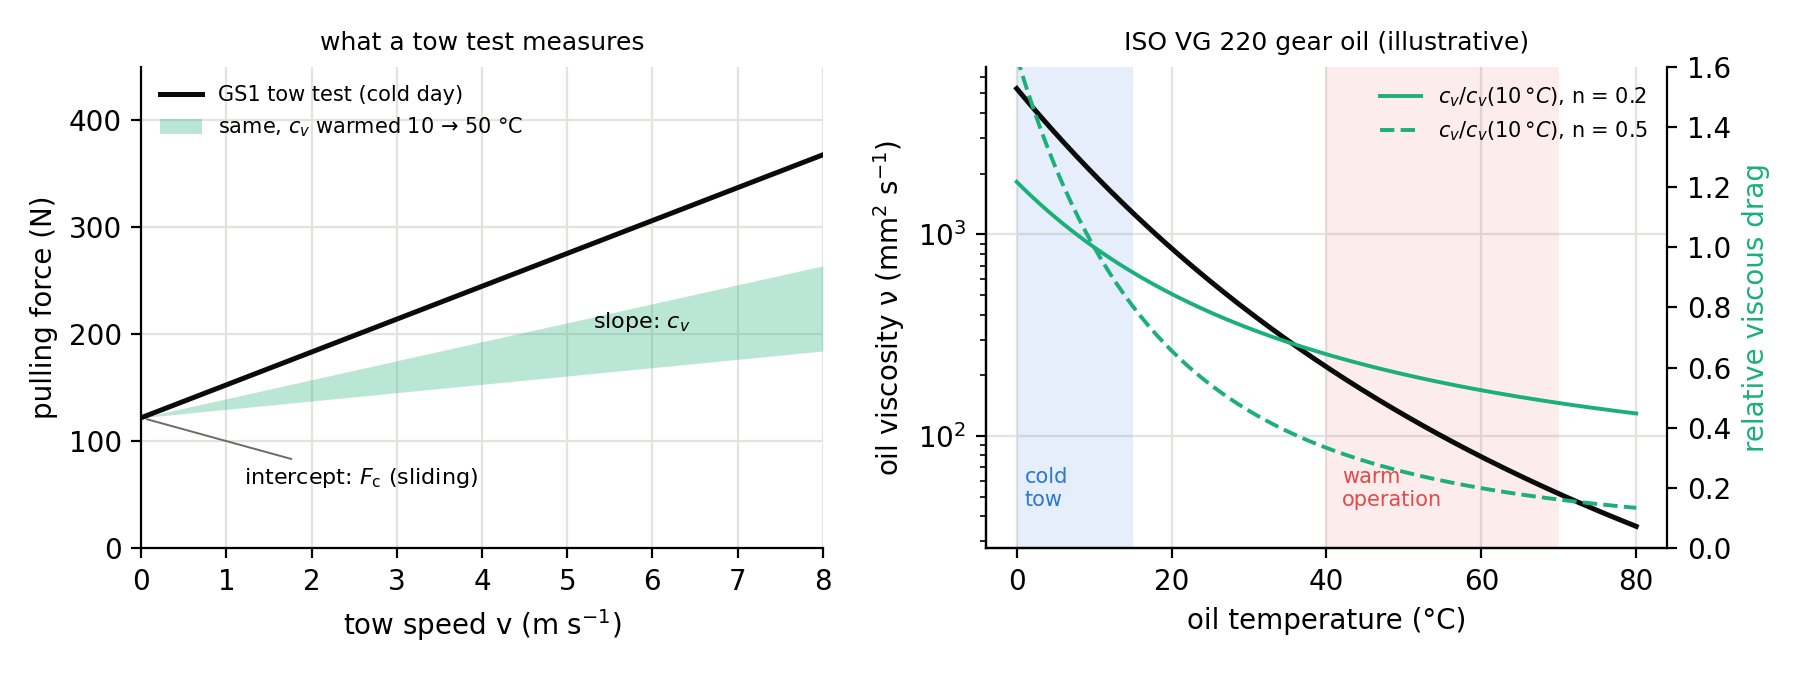
\includegraphics[width=0.95\textwidth]{drivetrain_tow_test.png}
\caption{Left: the tow-test law and the same law with its viscous slope
corrected from a cold to a warm gearbox. Right: viscosity of an ISO VG 220 gear
oil against temperature (Walther equation, \SI{220}{mm^2.s^{-1}} at
\SI{40}{\celsius}) and the resulting change of viscous drag for
$c_v \propto \nu^n$. The oil grade is illustrative.}
\label{fig:tow}
\end{figure}

\paragraph{Critique.} The tow test is the only measurement of this term, and it
has limits:
\begin{enumerate}
  \item \textbf{Cold oil biases it high.} Gear-oil viscosity changes very
    strongly with temperature: about ninefold between \SI{10}{\celsius} and
    \SI{40}{\celsius} for a VG 220 oil (Fig.~\ref{fig:tow}, right). Churning
    drag grows less than linearly with viscosity, roughly as $\nu^{n}$ with
    $n = 0.2$--0.5, so a gearbox at \SI{50}{\celsius} has a viscous drag of
    about 25--\SI{60}{\percent} of its value at \SI{10}{\celsius}. Seal
    friction also falls as the seals warm. For a warm gearbox the tow test
    is closer to an upper value than a central one.
  \item \textbf{It is a no-load test.} The tow tension is low, so the
    tension-proportional losses (belt, gear mesh, bearings) are absent. They
    come on top, as in Sect.~\ref{sec:est}.
  \item \textbf{The generator is included.} Electrically disconnected but
    turning, the generator contributes its bearings, fan and open-circuit iron
    losses (hysteresis behaves like a Coulomb term, eddy currents like a
    viscous one). These belong to the machine's drag. If an electrical
    efficiency used downstream already includes iron losses, they are counted
    twice.
  \item \textbf{Test details.} If the tow speeds stayed below the
    \SI{8}{m.s^{-1}} of fast reel-in, $c_v$ is extrapolated there. Tether
    dragging on the ground would add to the measured force. A single pull to
    breakaway, instead of steady speeds, would give the higher static
    friction.
\end{enumerate}

% ===========================================================================
\section{The measured energy chain of GS1}
\label{sec:gs1}

Fechner's AWEC 2011 talk \cite{fechner2011} reports an energy balance of GS1,
with four current sensors on the electrical side, for three consecutive pumping
cycles (test 104, flight 3; wind \SI{6}{m.s^{-1}} at \SI{6}{m}, maximum reel-out
and reel-in speeds 5.8 and \SI{8}{m.s^{-1}}, mean reel-out power
\SI{11.6}{kW}). Table~\ref{tab:gs1} regroups it per reel phase, and
Fig.~\ref{fig:gs1waterfall} follows cycle~1 from the tether to the electrical
output. The mechanical energies are sensor force times reel speed, so the
friction sits downstream of the sensor, as in Sect.~\ref{sec:sensor}. The
electrical losses include the motor controller.

\begin{table}[H]
\centering\small
\caption{GS1 energy per cycle, regrouped per reel phase from
\cite{fechner2011} (slide~13), in Wh. ``Terminals'' is the electrical energy
of the main machine. Efficiency is terminal over tether energy in reel-out and
tether over terminal energy in reel-in.}
\label{tab:gs1}
\begin{tabular}{llrrr}
\toprule
 & & Cycle 1 & Cycle 2 & Cycle 3 \\
\midrule
Reel-out & tether energy & 200 & 214 & 208 \\
 & friction & $-14$ & $-14$ & $-15$ \\
 & electrical losses & $-33$ & $-37$ & $-33$ \\
 & at the terminals & 153 & 163 & 160 \\
 & efficiency & \SI{76.5}{\percent} & \SI{76.2}{\percent} & \SI{76.9}{\percent} \\
\midrule
Reel-in & tether energy & 39 & 44 & 42 \\
 & friction & $+14$ & $+18$ & $+16$ \\
 & electrical losses & $+7$ & $+8$ & $+6$ \\
 & at the terminals & 60 & 70 & 64 \\
 & efficiency & \SI{65.0}{\percent} & \SI{62.9}{\percent} & \SI{65.6}{\percent} \\
\midrule
Auxiliaries & spindle motor / brakes, computers & 11 / 4 & 13 / 5 & 12 / 5 \\
\midrule
Net electrical & from the rows above & 78 & 75 & 79 \\
 & reported & 78 & 74 & 78 \\
\bottomrule
\end{tabular}
\end{table}

\begin{figure}[H]
\centering
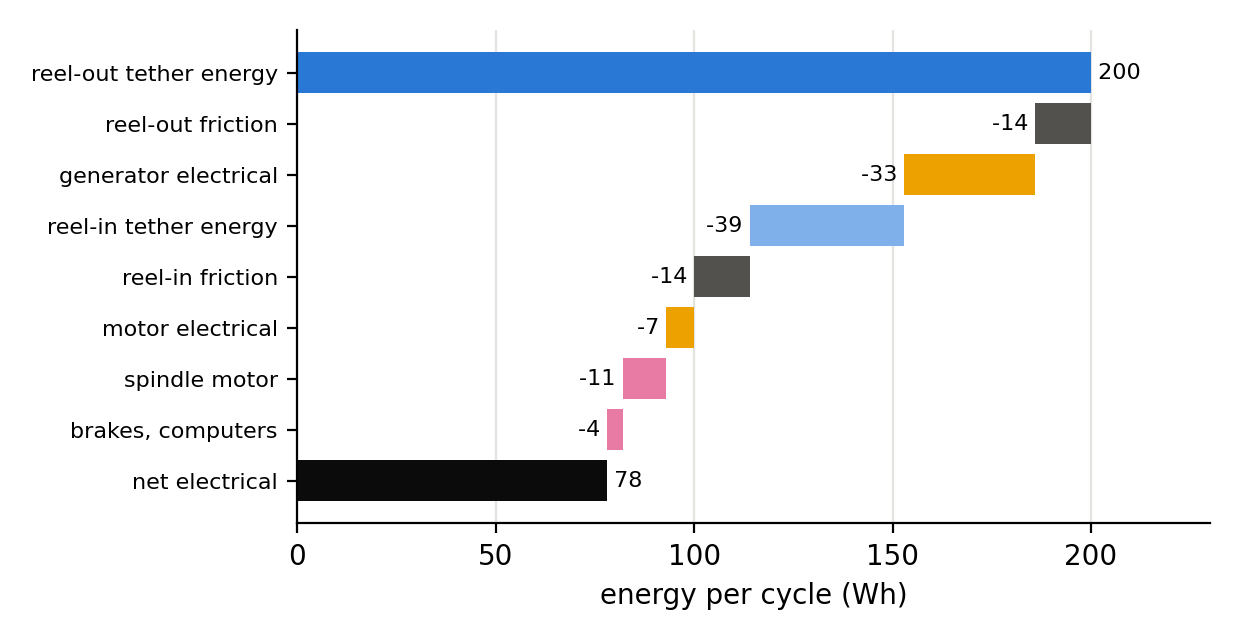
\includegraphics[width=0.8\textwidth]{drivetrain_gs1_waterfall.png}
\caption{GS1 cycle~1 from the reel-out tether energy to the net electrical
output, from \cite{fechner2011}.}
\label{fig:gs1waterfall}
\end{figure}

\begin{itemize}
  \item \textbf{Reel-out conversion is about \SI{76}{\percent}}: friction
    takes \SI{7}{\percent} of the tether energy, the generator and controller
    16--\SI{17}{\percent}.
  \item \textbf{Reel-in conversion is about \SI{65}{\percent}}, and the order
    is reversed: friction (14--\SI{18}{Wh}) is twice the electrical loss
    (6--\SI{8}{Wh}). The tension is low, so the copper losses, which grow with
    the square of the torque, are small, while the friction grows with the
    faster reel-in speed. This is the efficiency map of Fig.~\ref{fig:effmap}
    seen in measurements.
  \item \textbf{Friction is 17--\SI{20}{\percent} of the net mechanical
    energy}, and about half of it is spent in reel-in.
\end{itemize}

\paragraph{Consistency check.} With the talk's crest factors (1.71 out,
1.85 in) read as maximum over mean, the mean speeds are \SI{3.4}{m.s^{-1}} out
and \SI{4.3}{m.s^{-1}} in; with a period of about \SI{115}{s} and a duty cycle
of 0.53 the phases last about 61 and \SI{54}{s}. The tow-test law then gives
$(F_\mathrm{c}\bar v + c_v \bar v^2)\,t = \SI{13.0}{Wh}$ for reel-out and
\SI{16.5}{Wh} for reel-in, against the reported 14--15 and 14--\SI{18}{Wh}.
The agreement is close but probably circular: the current sensors measure the
machine's total loss, and splitting it into friction and electrical loss needs
a friction model, most likely this same law. Only the total (mechanical minus
electrical) is a measurement, and the tension-proportional mechanical losses
of Sect.~\ref{sec:est} are then booked as electrical.

\subsection{The same station in Fechner's thesis}
\label{sec:thesis}
Fechner's thesis \cite{fechner2016} analyses GS1 as the ``20~kW
demonstrator'' (Table~3.1 there: drum radius \SI{0.1615}{m}, \SI{4}{mm}
tether, \SI{8}{m.s^{-1}} reel speeds, \SI{4}{kN}, \SI{20}{kW} nominal
generator power; the talk says \SI{18}{kW}). It uses the same efficiency
chain under different names (Table~\ref{tab:eff}): the talk's $\eta_\mathrm{m}$
is the \emph{pumping efficiency} $\eta_\mathrm{p}$, $D\,\eta_\mathrm{p}$ is the
\emph{cycle efficiency} $\eta_\mathrm{cyc}$, and the talk's $\eta_\mathrm{e}$
splits into a gross electrical efficiency and a system efficiency for the
brakes and the spindle:
\begin{equation}
  \eta_\mathrm{e}^\mathrm{gro} =
  \frac{\eta_\mathrm{e,o}\,\eta_\mathrm{e,i}\,\eta_\mathrm{bat} - 1 + \eta_\mathrm{p}}
       {\eta_\mathrm{e,i}\,\eta_\mathrm{bat}\,\eta_\mathrm{p}} , \qquad
  \eta_\mathrm{tot} = D\,\eta_\mathrm{sys}\,\eta_\mathrm{e}^\mathrm{gro}\,\eta_\mathrm{p} ,
\end{equation}
with $\eta_\mathrm{e,o}$, $\eta_\mathrm{e,i}$ the generator and motor
efficiencies (friction included) and $\eta_\mathrm{bat}$ the battery's
(Eqs.~3.26 and 3.28 there). The form makes the point of
Sect.~\ref{sec:fruit} explicit: because the reel-in energy passes through
both machines and the battery, the gross electrical efficiency is always
lower than the generator's own.

\paragraph{Loss model.} The thesis models the generator loss as friction plus
copper loss (Eqs.~3.30--3.35 there):
$P_\mathrm{e,o} = P_\mathrm{m,o} - 3 R_\mathrm{g} I_\mathrm{o}^2 k - \tau_\mathrm{f,o}\,\omega$,
with the friction torque $\tau_\mathrm{f,o} = \tau_\mathrm{c} + c_\mathrm{v,f}\,\omega$
measured on the station (the tow test of Sect.~\ref{sec:tow}) and a factor $k$
for skin effect, stray-load and other losses not modelled explicitly. The
tension-proportional mechanical losses of Sect.~\ref{sec:est} (belt, gear
mesh, bearings) have no term of their own there; they would be absorbed in
$k$.

\paragraph{Numbers.} Table~\ref{tab:thesis} compares the talk with the
thesis's measured and simulated performance factors of the same station. They
agree within the spread between flights and wind conditions.

\begin{table}[H]
\centering\small
\caption{GS1 performance factors in the AWEC 2011 talk \cite{fechner2011} and
in the thesis \cite[Table~3.3 and Sect.~3.3.2]{fechner2016}.}
\label{tab:thesis}
\begin{tabular}{lrrr}
\toprule
 & Talk, measured & Thesis, measured & Thesis, simulated \\
\midrule
Pumping efficiency $\eta_\mathrm{p}$ ($\eta_\mathrm{m}$) & \SI{79.9}{\percent} & \SI{77}{\percent} & \SI{77}{\percent} \\
Duty cycle $D$ & \SI{53}{\percent} & \SI{56}{\percent} & \SI{46.8}{\percent} \\
Electrical efficiency & \SI{46.4}{\percent} & about \SI{54}{\percent} & -- \\
Total efficiency $\eta_\mathrm{tot}$ & \SI{19.6}{\percent} & \SI{21}{\percent} & \SI{18}{\percent} \\
Mean reel-out mechanical power & \SI{11.6}{kW} & \SI{14.1}{kW} & \SI{21.6}{kW} \\
Mean electrical output & \SI{2.29}{kW} & \SI{2.6}{kW} & \SI{4.0}{kW} \\
\bottomrule
\end{tabular}
\end{table}

\paragraph{Assumed against measured machine efficiencies.} For GS1 the thesis's
quasi-static model assumes a generator efficiency of \SI{80}{\percent}, a motor
efficiency of \SI{79}{\percent} and a battery efficiency of \SI{95}{\percent}
(Sect.~3.2.8 there). The talk's energy balance gives \SI{76.5}{\percent} in
reel-out and only \SI{65}{\percent} in reel-in (Table~\ref{tab:gs1}, friction
and controller included). The reel-in shortfall is what the thesis itself
explains in its Sect.~3.4: a machine's efficiency drops sharply at 10 or
\SI{20}{\percent} of its nominal power, and GS1 reeled in at about \SI{3}{kW}
on a \SI{20}{kW} machine.

\paragraph{The thesis's diagnosis.} The thesis attributes GS1's low electrical
efficiency to ``an asynchronous, squirrel cage generator \ldots{} together with
a very inefficient gearbox and a synchronous belt'' (Sect.~3.3.2 there), and
proposes a synchronous direct drive. That is the order of
Sect.~\ref{sec:fruit}: the machine first, then belt and gearbox.

% ===========================================================================
\section{Why the total efficiency is so low, and the low-hanging fruit}
\label{sec:fruit}

\paragraph{Which efficiency is which.} Several efficiencies appear in this note
and in \cite{fechner2011}; Table~\ref{tab:eff} lists what each one compares.
All energies are per cycle; ``tether energy'' is the sensor force times reel
speed, integrated over a phase.

\begin{table}[H]
\centering\small
\caption{Efficiencies used in this note. $E_\mathrm{o}$, $E_\mathrm{i}$: tether
energy in reel-out and reel-in; $E_\mathrm{m} = E_\mathrm{o} - E_\mathrm{i}$:
net mechanical energy; $E_\mathrm{e}$: net electrical energy, after the
auxiliaries; $t_\mathrm{o}$, $t_\mathrm{i}$: phase durations. ``Thesis'': the name in
\cite{fechner2016} (Sect.~\ref{sec:thesis}). GS1 values from \cite{fechner2011}.}
\label{tab:eff}
\begin{tabularx}{\textwidth}{llXr}
\toprule
Name & Thesis & Compares & GS1 \\
\midrule
Mechanical drivetrain efficiency (Fig.~\ref{fig:effmap}) & -- & shaft over tether power at one instant (reel-in: the inverse); the mechanical chain only & -- \\
Duty cycle $D$ & $D$ & $t_\mathrm{o}/(t_\mathrm{o}+t_\mathrm{i})$; a time share, not a loss & \SI{53}{\percent} \\
Mechanical cycle efficiency $\eta_\mathrm{m}$ & $\eta_\mathrm{p}$ & $E_\mathrm{m}/E_\mathrm{o}$: how much reel-out work is not spent on the reel-in; set by the kite and flight, not the drivetrain & \SI{79.9}{\percent} \\
Electrical efficiency $\eta_\mathrm{e}$ & $\eta_\mathrm{e}^\mathrm{gro}\,\eta_\mathrm{sys}$ & $E_\mathrm{e}/E_\mathrm{m}$: net electrical over net mechanical energy; includes friction, machine and controller losses in both phases, and the auxiliaries & \SI{46.4}{\percent} \\
Total efficiency $\eta_\mathrm{tot}$ & $\eta_\mathrm{tot}$ & $D\,\eta_\mathrm{m}\,\eta_\mathrm{e}$: cycle-mean electrical power over the mean reel-out mechanical power & \SI{19.6}{\percent} \\
Energy share & -- & $E_\mathrm{e}/E_\mathrm{o} = \eta_\mathrm{m}\,\eta_\mathrm{e}$: net electrical over reel-out tether energy & \SI{39}{\percent} \\
\bottomrule
\end{tabularx}
\end{table}

\paragraph{The headline number.} The talk's \SI{19.6}{\percent} total
efficiency is $0.53 \times 0.799 \times 0.464$. The duty cycle in it is not lost
energy: it says the station is idle as a generator during reel-in, which
matters for the installed power and its cost, not for the energy. In energy
terms, \SI{78}{Wh} of \SI{200}{Wh}, or \SI{39}{\percent} of the reel-out tether
energy, reached the electrical output. That is still poor.

\paragraph{The culprits.} Of the \SI{200}{Wh} reel-out tether energy of
cycle~1 (Fig.~\ref{fig:gs1waterfall}):
\begin{enumerate}
  \item \textbf{Electrical conversion, \SI{40}{Wh} (\SI{20}{\percent}).} The
    largest item, mostly in reel-out (\SI{33}{Wh}): the generator and its
    controller convert about \SI{82}{\percent} of the shaft energy. One machine
    serves both directions over a wide torque and speed range, and at part load
    its fixed losses weigh heavily.
  \item \textbf{Reel-in tether work, \SI{39}{Wh} (\SI{20}{\percent}).} The
    work done pulling the kite back. This is set by the kite and the flight
    strategy, not the station.
  \item \textbf{Friction, \SI{28}{Wh} (\SI{14}{\percent}).} Half of it in
    reel-in, where the speed is high and the load low.
  \item \textbf{Auxiliaries, \SI{15}{Wh} (\SI{8}{\percent}).} The spindle
    motor (200--\SI{600}{W}) and the brakes and computers (about \SI{150}{W})
    run all the time.
\end{enumerate}

\paragraph{Reel-in energy is paid twice.} Every watt-hour the motor spends in
reel-in was first generated in reel-out and passed through the generator. On
GS1, \SI{1}{Wh} of reel-in tether work costs $1/0.65 = \SI{1.5}{Wh}$ at the
terminals, which took $1.5/0.765 \approx \SI{2}{Wh}$ of reel-out tether energy.
The same multiplier applies to the reel-in friction. Reducing the reel-in work
and the reel-in friction therefore pays about double.

\paragraph{Levers.} Figure~\ref{fig:fruit} applies each lever alone to GS1
cycle~1. The effects are illustrative: they rest on the stated assumptions,
not on measurements.
\begin{itemize}
  \item \textbf{Brake holding current} (cheap). Spring-applied brakes draw
    current the whole time they are released. An economiser drops the holding
    current to about a third after pull-in. Assumed \SI{4}{Wh} $\to$
    \SI{1}{Wh} per cycle: $+\SI{3}{Wh}$.
  \item \textbf{Spindle drive} (cheap to moderate). GS1's spindle moved the
    drum and the generator, the heaviest parts of the station, through a worm
    drive, which slides rather than rolls and typically transmits only
    40--\SI{70}{\percent} of its input. Moving only a light guide pulley, with
    a ball or lead screw and a small motor, and only while the tether moves,
    needs a fraction of that. Assumed \SI{11}{Wh} $\to$ \SI{4}{Wh}:
    $+\SI{7}{Wh}$.
  \item \textbf{Oil and seals} (cheap). The lowest oil viscosity the gearbox
    allows, the correct fill level (over-filling raises churning), a warm-up
    before flying, and low-friction seals. Assumed viscous drag
    $-\SI{30}{\percent}$ and seal drag $-\SI{1.5}{Wh}$ per phase:
    $+\SI{7}{Wh}$.
  \item \textbf{Reel-in strategy} (free, in software). Fly the reel-in more
    depowered and at a better elevation, and choose the reel-in speed with
    the friction in view: a faster reel-in shortens the cycle but pays
    friction that grows with speed. AWETrim's cycle optimiser can maximise the
    shaft power instead of the tether power (Sect.~\ref{sec:objective}); on
    the LEI-V3 cycles that cuts the reel-in work by 7--\SI{25}{\percent} but
    gains only about \SI{1}{\percent} at the shaft. Assumed reel-in tether
    work $-\SI{25}{\percent}$: $+\SI{10}{Wh}$.
  \item \textbf{Machine and inverter} (not cheap, largest). A
    permanent-magnet machine with a modern inverter reaches about
    \SI{94}{\percent} in each direction at these loads, against the 82 and
    \SI{88}{\percent} of GS1's machine and controller: $+\SI{25}{Wh}$.
  \item \textbf{Drivetrain architecture} (a redesign). Remove the belt and the
    gearbox with a direct drive, and size the machines for their phases: a
    high-torque generator for reel-out and a smaller, faster motor for
    reel-in, so that neither runs at a few percent of its rating. A clutch
    decouples the generator during reel-in, so its friction is not paid
    there. This is the design the thesis proposes for a \SI{53.5}{kW} station
    \cite[Sect.~3.4]{fechner2016}; with \SI{90}{\percent} machines it
    simulates a gross electrical efficiency of 85--\SI{88}{\percent} and a
    total efficiency of \SI{57}{\percent}. It is not in Fig.~\ref{fig:fruit}.
\end{itemize}
Together the four cheap levers raise the net output from 78 to about
\SI{105}{Wh} per cycle, a third more; with the machine upgrade it is about
\SI{131}{Wh}, \SI{66}{\percent} of the reel-out tether energy instead of
\SI{39}{\percent}. The pulleys and the drum are not worth touching: they cost a
few percent at most.

\begin{figure}[H]
\centering
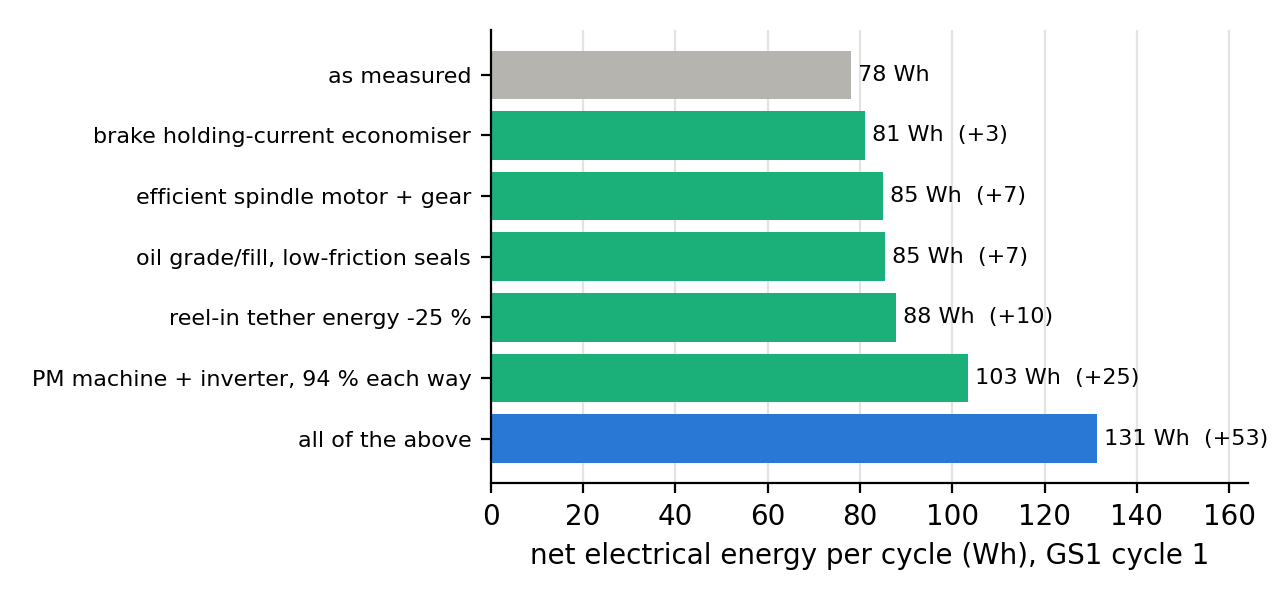
\includegraphics[width=0.8\textwidth]{drivetrain_gs1_improvements.png}
\caption{Net electrical energy of GS1 cycle~1 as measured and with each lever
applied alone (assumptions in the text). Green: the levers; blue: all
together.}
\label{fig:fruit}
\end{figure}

% ===========================================================================
\section{What would pin such an estimate down}
For any ground station, these measurements would replace the assumptions above:
\begin{enumerate}
  \item \textbf{A warm no-load constant-speed test}: tether slack, motor
    driving at several steady speeds in both directions up to the reel-in
    maximum, torque logged, after the gearbox has reached its operating
    temperature. This measures $F_\mathrm{c}$ and $c_v$, the dominant term,
    directly; repeating it with the motor decoupled separates machine and
    gearbox.
  \item \textbf{The gearbox oil grade and its sump temperature in operation},
    to correct a cold test.
  \item \textbf{The gearbox and belt datasheets}: efficiency against load and
    speed, oil fill and seal type.
  \item \textbf{Bearing types and sizes} of the pulleys and the drum.
  \item \textbf{A second force measurement at the drum}, for example from the
    motor torque on a calibrated drive. Its difference to the sensor on the
    last pulley would isolate the downstream losses.
  \item \textbf{An energy balance like Table~\ref{tab:gs1}}, with mechanical
    and electrical sides measured independently, including the auxiliaries.
\end{enumerate}

\begin{thebibliography}{9}
\bibitem{fechner2011}
U.~Fechner, \emph{Performance factors for HAWP systems in pumping operation},
presentation, Airborne Wind Energy Conference (AWEC) 2011, KU Leuven, 2011.
\bibitem{fechner2016}
U.~Fechner, \emph{A Methodology for the Design of Kite-Power Control Systems},
PhD thesis, Delft University of Technology, 2016,
\url{https://doi.org/10.4233/uuid:85efaf4c-9dce-4111-bc91-7171b9da4b77}.
\bibitem{skf}
SKF, \emph{Rolling bearings} (general catalogue), section on bearing friction
and the simplified friction-torque model.
\bibitem{feyrer}
K.~Feyrer, \emph{Wire Ropes: Tension, Endurance, Reliability}, 2nd ed.,
Springer, 2015.
\bibitem{iso14179}
ISO/TR 14179-1:2001, \emph{Gears --- Thermal capacity --- Part 1: Rating gear
drives with thermal equilibrium at 95\,\textdegree C sump temperature}.
\bibitem{iec60034}
IEC 60034-2-1, \emph{Rotating electrical machines --- Part 2-1: Standard
methods for determining losses and efficiency from tests}.
\end{thebibliography}

\end{document}
